%% (Master) Thesis template
% Template version used: v1.4
%
% Largely adapted from Adrian Nievergelt's template for the ADPS
% (lecture notes) project.



%% We use the memoir class because it offers a many easy to use features.
\documentclass[11pt,a4paper,table,hidelinks]{memoir}  % Remove "hidelinks" for red boxes around hyperlinks

%% Packages
%% ========

%% LaTeX Font encoding -- DO NOT CHANGE
\usepackage[OT1]{fontenc}

%% Babel provides support for languages.  'english' uses British
%% English hyphenation and text snippets like "Figure" and
%% "Theorem". Use the option 'ngerman' if your document is in German.
%% Use 'american' for American English.  Note that if you change this,
%% the next LaTeX run may show spurious errors.  Simply run it again.
%% If they persist, remove the .aux file and try again.
\usepackage[english]{babel}

%% Input encoding 'utf8'. In some cases you might need 'utf8x' for
%% extra symbols. Not all editors, especially on Windows, are UTF-8
%% capable, so you may want to use 'latin1' instead.
\usepackage[utf8]{inputenc}

%% This changes default fonts for both text and math mode to use Herman Zapfs
%% excellent Palatino font.  Do not change this.
%\usepackage[sc]{mathpazo}

%% The AMS-LaTeX extensions for mathematical typesetting.  Do not
%% remove.
\usepackage{amsmath,amssymb,amsfonts,mathrsfs}

%% NTheorem is a reimplementation of the AMS Theorem package. This
%% will allow us to typeset theorems like examples, proofs and
%% similar.  Do not remove.
%% NOTE: Must be loaded AFTER amsmath, or the \qed placement will
%% break
\usepackage[amsmath,thmmarks]{ntheorem}

%% LaTeX' own graphics handling
\usepackage{graphicx}

%% We unfortunately need this for the Rules chapter.  Remove it
%% afterwards; or at least NEVER use its underlining features.
\usepackage{soul}

%% This allows you to add .pdf files. It is used to add the
%% declaration of originality.
\usepackage{pdfpages}

\newenvironment{conditions}
  {\par\vspace{\abovedisplayskip}\noindent\begin{tabular}{>{$}l<{$} @{${}={}$} l}}
  {\end{tabular}\par\vspace{\belowdisplayskip}}

%% Some more packages that you may want to use.  Have a look at the
%% file, and consult the package docs for each.
%% See the TeXed file for more explanations

%% [OPT] Multi-rowed cells in tabulars
%\usepackage{multirow}

%% [REC] Intelligent cross reference package. This allows for nice
%% combined references that include the reference and a hint to where
%% to look for it.
\usepackage{varioref}

%% [OPT] Easily changeable quotes with \enquote{Text}
%\usepackage[german=swiss]{csquotes}

%% [REC] Format dates and time depending on locale
\let\ordinal\relax %% prevent warning
\usepackage{datetime}

%% [OPT] Provides a \cancel{} command to stroke through mathematics.
%\usepackage{cancel}

%% [NEED] This allows for additional typesetting tools in mathmode.
%% See its excellent documentation.
\usepackage{mathtools}

%% [NEED] Conditional commands
\usepackage{ifthen}

%% [OPT] Manual large braces or other delimiters.
%\usepackage{bigdelim, bigstrut}

%% [REC] Alternate vector arrows. Use the command \vv{} to get scaled
%% vector arrows.
\usepackage[h]{esvect}

%% [NEED] Some extensions to tabulars and array environments.
\usepackage{array}

%% [OPT] Postscript support via pstricks graphics package. Very
%% diverse applications.
%\usepackage{pstricks,pst-all}

%% [?] This seems to allow us to define some additional counters.
%\usepackage{etex}

%% [ADV] XY-Pic to typeset some matrix-style graphics
%\usepackage[all]{xy}

%% [OPT] This is needed to generate an index at the end of the
%% document.
%\usepackage{makeidx}

%% [OPT] Fancy package for source code listings.  The template text
%% needs it for some LaTeX snippets; remove/adapt the \lstset when you
%% remove the template content.
\usepackage{listings}
% \lstset{language=TeX,basicstyle={\normalfont\ttfamily}}

%% [REC] Fancy character protrusion.  Must be loaded after all fonts.
%\usepackage[activate]{pdfcprot}

%% [REC] Nicer tables.  Read the excellent documentation.
\usepackage{booktabs}

%% [OPT] Package for adding TODOs.
\usepackage{todonotes}

%% [OPT] Package to define and use acronyms
\usepackage[nolist,nohyperlinks,smaller]{acronym}

\usepackage{caption}
\usepackage{subcaption}
\expandafter\def\csname ver@subfig.sty\endcsname{}
 

%% Our layout configuration.  DO NOT CHANGE.
%% Memoir layout setup

%% NOTE: You are strongly advised not to change any of them unless you
%% know what you are doing.  These settings strongly interact in the
%% final look of the document.

% Dependencies
%\usepackage{ETHlogo}

% use helvetica as default font:
\usepackage[scaled]{helvet}
%\renewcommand\familydefault{\sfdefault} 

% Turn extra space before chapter headings off.
\setlength{\beforechapskip}{0pt}

\nonzeroparskip
\parindent=0pt
\defaultlists

% Chapter style redefinition
\makeatletter

\makepagestyle{headerWPageNr}% Create headerWPageNr style
\if@twoside
  \copypagestyle{headerWPageNr}{Ruled}
  \copypagestyle{chapter}{Ruled}
\else
  \copypagestyle{headerWPageNr}{ruled}
  \copypagestyle{chapter}{ruled}
\fi
% chapter pages have no header and center page number in footer:
\makeoddhead{chapter}{}{}{}
\makeevenhead{chapter}{}{}{}
\makeoddfoot{chapter}{}{\thepage}{}
\makeevenfoot{chapter}{}{\thepage}{}
\makeheadrule{chapter}{\textwidth}{0pt}

% all other pages have page number and chapter or section name in header without footer:
\makeoddhead{headerWPageNr}{\rightmark}{}{\thepage}
\makeevenhead{headerWPageNr}{\thepage}{}{\leftmark}
\makeoddfoot{headerWPageNr}{}{}{}
\makeevenfoot{headerWPageNr}{}{}{}
\pagestyle{headerWPageNr}% Set page style to headerWPageNr


\makechapterstyle{bianchimod}{%
  \copypagestyle{abstract}{empty}
  \copypagestyle{acknowledgement}{empty}
  \chapterstyle{default}
  \renewcommand*{\chapnamefont}{\normalfont\Large\sffamily}
  \renewcommand*{\chapnumfont}{\normalfont\Large\sffamily}
  \renewcommand*{\printchaptername}{%
    \chapnamefont\centering\@chapapp}
  \renewcommand*{\printchapternum}{\chapnumfont {\thechapter}}
  \renewcommand*{\chaptitlefont}{\normalfont\huge\sffamily}
  \renewcommand*{\printchaptertitle}[1]{%
    \hrule\vskip\onelineskip \centering \chaptitlefont\textbf{\vphantom{gyM}##1}\par}
  \renewcommand*{\afterchaptertitle}{\vskip\onelineskip \hrule\vskip
    \afterchapskip}
  \renewcommand*{\printchapternonum}{%
    \vphantom{\chapnumfont {9}}\afterchapternum}}
  
\makechapterstyle{bianchimod2}{%
  \renewenvironment{abstract}{\chapter*{\abstractname}}{}
  \newenvironment{acknowledgement}{\chapter*{Acknowledgement}}{}
  \chapterstyle{default}
  \definecolor{ChapGrey}{rgb}{0.6,0.6,0.6}
  \newcommand{\LargeFont}{% Needs a ’stretchable’ font
  	\usefont{\encodingdefault}{\sfdefault}{b}{n}%
    \fontsize{100}{0}\selectfont\color{ChapGrey}}
  \renewcommand*{\chapnumfont}{\LargeFont}
  \renewcommand*{\printchaptername}{\raggedleft}
  \renewcommand*{\printchapternum}{\chapnumfont {\thechapter}}
  \renewcommand*{\chaptitlefont}{\normalfont\Huge\sffamily\color{black}}
  \renewcommand*{\printchaptertitle}[1]{%
    \raggedleft \chaptitlefont\textbf{\vphantom{gyM}##1}\par}}

% Use the newly defined style
\chapterstyle{bianchimod2}

\setsecheadstyle{\Large\bfseries\sffamily}
\setsubsecheadstyle{\large\bfseries\sffamily}
\setsubsubsecheadstyle{\bfseries\sffamily}
\setparaheadstyle{\normalsize\bfseries\sffamily}
\setsubparaheadstyle{\normalsize\itshape\sffamily}
\setsubparaindent{0pt}

% Set captions to a more separated style for clearness
\captionnamefont{\sffamily\bfseries\footnotesize}
\captiontitlefont{\sffamily\footnotesize}
\setlength{\intextsep}{16pt}
\setlength{\belowcaptionskip}{1pt}

% Set section and TOC numbering depth to subsection
\setsecnumdepth{subsection}
\settocdepth{subsection}

% definitions for titlepage
\def\@advisor{}
\newcommand{\advisor}[1]{\def\@advisor{#1}}
\def\@supervisor{}
\newcommand{\supervisor}[1]{\def\@supervisor{#1}}
\def\@group{}
\newcommand{\group}[1]{\def\@group{#1}}
\def\@institute{}
\newcommand{\institute}[1]{\def\@institute{#1}}
\def\@department{}
\newcommand{\department}[1]{\def\@department{#1}}
\def\@school{}
\newcommand{\school}[1]{\def\@school{#1}}
\def\@thesistype{}
\newcommand{\thesistype}[1]{\def\@thesistype{#1}}
\def\@email{}
\newcommand{\email}[1]{\def\@email{#1}}

%% Title page adjustments
% the following definition (either 0 or 1) controls the title page's layout:
\def\centeredtitlepage{0}
\if\centeredtitlepage1
	% default title page from cadmo template
	\newcommand{\maketitlepage}{
		\begin{titlingpage}
  			\calccentering{\unitlength}
  			\begin{adjustwidth*}{\unitlength-24pt}{-\unitlength-24pt}
    		\maketitle
  			\end{adjustwidth*}
		\end{titlingpage}
	}
	\pretitle{\vspace{0pt plus 0.7fill}\begin{center}\HUGE\sffamily\bfseries}
	\posttitle{\end{center}\par}
	\preauthor{\par\begin{center}\let\and\\\Large\sffamily}
	\postauthor{\end{center}}
	\predate{\par\begin{center}\Large\sffamily}
	\postdate{\end{center}}

	\renewcommand{\maketitlehooka}{\noindent\ETHlogo[2in]}

	\renewcommand{\maketitlehookb}{\vspace{1in}%
  		\par\begin{center}\Large\sffamily\@thesistype\end{center}}

	\renewcommand{\maketitlehookd}{%
  		\vfill\par
  			\begin{flushright}
    			\sffamily
    			Advisors: \@supervisor, \@advisor\par
    			\@department, \@school
  			\end{flushright}
	}

\else
	% alternative title page (right-aligned)
	\newcommand{\maketitlepage}{
		\begin{titlingpage}
			\titlestyleright
		\end{titlingpage}
	}
	\newcommand*\titlestyleright{
		\thispagestyle{empty}
		\begin{minipage}[c]{0.35\linewidth}
			\vspace{0pt}
			\hfuzz=5.0pt
			
\includegraphics[width=0.9\linewidth]{images/ost_logo_de_rgb-eps-converted-to}
		\end{minipage}
		%
		\begin{minipage}[c]{0.4\linewidth}
			\vspace{0pt}
			\-\
		\end{minipage}
		%
		\begin{minipage}[c]{0.25\linewidth}
			\vspace{0pt}
			\hfuzz=6.0pt
			    \hspace*{-1.7cm} 
			        
\includegraphics[width=1.5\linewidth]{images/icai_logo}
		\end{minipage}
		\vspace{2cm}
		\sffamily
		\vspace*{\stretch{6}}
		\begin{flushright}
		{\Huge\sffamily\bfseries\@title\par}
		\par\noindent\rule[-1ex]{\linewidth}{2pt}\par
		\vspace{0.5cm}
		\emph{\huge\sffamily\@thesistype}
		\vspace{2cm}\par
		{\LARGE\sffamily\bfseries Florian Baumgartner}\par
		{\sffamily\ \href{mailto:florian.baumgartner@ost.ch}{florian.baumgartner@ost.ch}}\par
		\vspace{0.5cm}
		{\LARGE\sffamily\bfseries Alain Keller}\par
		{\sffamily\ \href{mailto:alain.keller@ost.ch}{alain.keller@ost.ch}}\par
		\vspace{1cm}
    	{\large\textbf{Advisor}\par
    		\@advisor\par}
    	\vspace{0.5cm}
    	{\large\textbf{Examiner}\par
    		\@supervisor\par}
    	\vspace{1cm}
    	{\@institute\par
        	\@school\par}
    	\vspace{1cm}
    	{\normalsize\@date\par}
		\end{flushright}
		\vspace{\stretch{1}}
		\noindent
		\pagebreak 
    	\sffamily
    	\thispagestyle{empty} 
	}
\fi

%Change margins
\setlrmarginsandblock{3.5cm}{3cm}{*}
\setulmarginsandblock{3cm}{*}{1}
\checkandfixthelayout

\setlength{\droptitle}{-48pt}

\makeatother

% This defines how theorems should look. Best leave as is.
\theoremstyle{plain}
\setlength\theorempostskipamount{0pt}

%%% Local Variables:
%%% mode: latex
%%% TeX-master: "thesis"
%%% End:


%% Theorem environments.  You will have to adapt this for a German
%% thesis.
%% Theorem-like environments

%% This can be changed according to language. You can comment out the ones you
%% don't need.

\numberwithin{equation}{chapter}

%% German theorems
%\newtheorem{satz}{Satz}[chapter]
%\newtheorem{beispiel}[satz]{Beispiel}
%\newtheorem{bemerkung}[satz]{Bemerkung}
%\newtheorem{korrolar}[satz]{Korrolar}
%\newtheorem{definition}[satz]{Definition}
%\newtheorem{lemma}[satz]{Lemma}
%\newtheorem{proposition}[satz]{Proposition}

%% English variants
\newtheorem{theorem}{Theorem}[chapter]
\newtheorem{example}[theorem]{Example}
\newtheorem{remark}[theorem]{Remark}
\newtheorem{corollary}[theorem]{Corollary}
\newtheorem{definition}[theorem]{Definition}
\newtheorem{lemma}[theorem]{Lemma}
\newtheorem{proposition}[theorem]{Proposition}

%% Proof environment with a small square as a "qed" symbol
\theoremstyle{nonumberplain}
\theorembodyfont{\normalfont}
\theoremsymbol{\ensuremath{\square}}
\newtheorem{proof}{Proof}
%\newtheorem{beweis}{Beweis}


%% Helpful macros.
%% Custom commands
%% ===============

%% Special characters for number sets, e.g. real or complex numbers.
\newcommand{\C}{\mathbb{C}}
\newcommand{\K}{\mathbb{K}}
\newcommand{\N}{\mathbb{N}}
\newcommand{\Q}{\mathbb{Q}}
\newcommand{\R}{\mathbb{R}}
\newcommand{\Z}{\mathbb{Z}}
\newcommand{\X}{\mathbb{X}}

%% Fixed/scaling delimiter examples (see mathtools documentation)
\DeclarePairedDelimiter\abs{\lvert}{\rvert}
\DeclarePairedDelimiter\norm{\lVert}{\rVert}

%% Use the alternative epsilon per default and define the old one as \oldepsilon
\let\oldepsilon\epsilon
\renewcommand{\epsilon}{\ensuremath\varepsilon}

%% Also set the alternate phi as default.
\let\oldphi\phi
\renewcommand{\phi}{\ensuremath{\varphi}}

\makeatletter
\newcommand{\thickhline}{%
    \noalign {\ifnum 0=`}\fi \hrule height 2pt
    \futurelet \reserved@a \@xhline
}
\newcolumntype{"}{@{\hskip\tabcolsep\vrule width 2pt\hskip\tabcolsep}}
\makeatother

\newcolumntype{P}[1]{>{\centering\arraybackslash}p{#1}}

%% This allow the usage of dashed and dotted lines in tables
\usepackage{arydshln}
\usepackage{hhline}
\usepackage{mathrsfs}
\usepackage{lscape}
\usepackage{siunitx}
\usepackage{caption}
%\usepackage{subcaption}  % Removed this because of subfig
% \usepackage{subfig}
\usepackage{textcomp}

\DeclareCaptionFont{fcaption}{\footnotesize}
%\captionsetup{labelfont={sf, bf}, textfont=sf, font=fcaption}
%\captionsetup[sub]{font=fcaption,labelfont={sf}}

%% Make document internal hyperlinks wherever possible. (TOC, references)
%% This MUST be loaded after varioref, which is loaded in 'extrapackages'
%% above.  We just load it last to be safe.
\usepackage[linkcolor=black,colorlinks=false,citecolor=black,filecolor=black]{hyperref}
\usepackage[capitalize, noabbrev]{cleveref}

%\usepackage[showframe]{geometry}% http://ctan.org/pkg/geometry
%\usepackage{lipsum}% http://ctan.org/pkg/lipsum
%\usepackage{graphicx}% http://ctan.org/pkg/graphicx

\usepackage{setspace}
\usepackage{parskip}
\usepackage{wrapfig}
\usepackage{verbatimbox}
\usepackage{bold-extra}
\usepackage{graphbox}
\usepackage{setspace}
\usepackage{framed}
\usepackage{bm}

\NewDocumentCommand{\codeword}{v}{%
\texttt{\textcolor{black}{#1}}%
}
\lstset{language=C,keywordstyle={\bfseries \color{blue}}}

%% Suppress warnings, kind of hack..
\usepackage{silence}
\WarningFilter{glossaries}{Overriding \printglossary}
\WarningFilter{glossaries}{Overriding `theglossary'}
%% Important: Must be last import package, otherwise hyperlinks do not work?!
\usepackage[acronym]{glossaries}

%% Document information
%% ====================

\title{Acoustic Source Localization using a Microphone Array}
\author{}
\email{}
\thesistype{Project Thesis}
\advisor{Hannes Badertscher}
% \supervisor{None}
\group{}
\institute{Interdisciplinary Center for Artificial Intelligence}
\department{MSE}
\school{Eastern Switzerland University of Applied Sciences}
\date{January 2024}

\makeglossaries
\pagenumbering{Roman}
\apptocmd{\sloppy}{\hbadness 4000\relax}{}{}  %% Suppress Underfull \vbox warning for bibliography
\begin{document}
\frontmatter

%% Title page is autogenerated from document information above.  DO
%% NOT CHANGE.
\hfuzz=6.0pt \maketitlepage

%% The abstract of your thesis.  Edit the file as needed.
\begin{abstract}
    Lorem ipsum dolor sit amet, consetetur sadipscing elitr, 
    sed diam nonumy eirmod tempor invidunt ut labore et dolore magna aliquyam erat, 
    sed diam voluptua. At vero eos et accusam et justo duo dolores et ea rebum. 
    Stet clita kasd gubergren, no sea takimata sanctus est Lorem ipsum dolor sit amet. 
    Lorem ipsum dolor sit amet, consetetur sadipscing elitr, 
    ed diam nonumy eirmod tempor invidunt ut labore et dolore magna aliquyam erat, 
    sed diam voluptua. 
    At vero eos et accusam et justo duo dolores et ea rebum. 
    Stet clita kasd gubergren, no sea takimata sanctus est Lorem ipsum dolor sit amet.
\end{abstract}

\begin{acknowledgement}
We take this opportunity to express gratitude to all of the people that supported us in this thesis.
\end{acknowledgement}

%% reset acronym usage:

%% TOC with the proper setup, do not change.
\cleartorecto
{
	\linespread{1.03}\selectfont{}
	\tableofcontents*       % This asterisk is important to prevent listing "Contents" in the table of contents
}
\mainmatter
\renewcommand{\thefigure}{\thechapter.\arabic{figure}}

\newglossaryentry{arduino}
{
	name=Arduino,
	description={Is an open-source company providing software libraries and microcontroller kits}
}

\newglossaryentry{openai-codex}
{
	name=OpenAI Codex,
	description={Is an artificial intelligence model developed by OpenAI. It parses natural language and generates code in response}
}

\newglossaryentry{adafruit}
{
	name=Adafruit,
	description={Adafruit Industries is an open-source hardware company based in New York City that designs and manufactures electronic development boards}
}

\newacronym{ssl}{SSL}{Sound Source Localization}
\newacronym{tdoa}{TDOA}{Time Differnece of Arrival}
\newacronym{doa}{DOA}{Direction of Arrival}
\newacronym{wlan}{WLAN}{Wireless LAN}
\newacronym{lan}{LAN}{Local Area Network}
\newacronym{nac}{NAC}{Network Access Control}
\newacronym{iot}{IoT}{Internet of Things}
\newacronym{fms}{FMS}{Fleet Management System}
\newacronym{can}{CAN}{Controller Area Network}
\newacronym{twai}{TWAI}{Two Wire Automotive Interface}
\newacronym{usb}{USB}{Universal Serial Bus}
\newacronym{imu}{IMU}{Inertial Measurement Unit}
\newacronym{pcb}{PCB}{Printed Circuit Board}
\newacronym{soc}{SoC}{System on a Chip}
\newacronym{led}{LED}{Light-Emitting Diode}
\newacronym{gnss}{GNSS}{Global Navigation Satellite System}
\newacronym{sae}{SAE}{Society of Automotive Engineers}
\newacronym{ptc}{PTC}{Positive Temperature Coefficient}
\newacronym{dfu}{DFU}{Device Firmware Update}
\newacronym{jtag}{JTAG}{Joint Test Action Group}
\newacronym{rf}{RF}{Radio Frequency}
\newacronym{phy}{PHY}{Physical Layer}
\newacronym{tcp}{TCP}{Transmission Control Protocol}
\newacronym{ip}{IP}{Internet Protocol}
\newacronym{spi}{SPI}{Serial Peripheral Interface}
\newacronym{cad}{CAD}{Computer Aided Design}
\newacronym{mit}{MIT}{Massachusetts Institute of Technology}
\newacronym{fat}{FAT}{File Allocation Table}
\newacronym{msc}{MSC}{Mass Storage Controller}
\newacronym{cdc}{CDC}{Communications Device Class}
\newacronym{vcp}{VCP}{Virtual COM Port}
\newacronym{json}{JSON}{JavaScript Object Notation}
\newacronym{ssid}{SSID}{Service Set Identifier}
\newacronym{ap}{AP}{Access Point}
\newacronym{rtr}{RTR}{Remote Transmission Request}
\newacronym{crc}{CRC}{Cyclic Redundancy Check}
\newacronym{pgn}{PGN}{Parameter Group Number}
\newacronym{http}{HTTP}{Hypertext Transfer Protocol}
\newacronym{udp}{UDP}{User Datagram Protocol}
\newacronym{ascii}{ASCII}{American Standard Code for Information Interchange}
\newacronym{ppm}{ppm}{parts per million}
\newacronym{gui}{GUI}{Graphical User Interface}
\newacronym{ide}{IDE}{Integrated Development Environment}
\newacronym{i2c}{I\textsuperscript{2}C}{Inter-Integrated Circuit}
\newacronym{din}{DIN}{Deutsches Institut für Normung}
\newacronym{dc}{DC}{Direct Current}
\newacronym{cm}{CM}{Common-Mode}
\newacronym{cpu}{CPU}{Central Processing Unit}
\newacronym{ieee}{IEEE}{Institute of Electrical and Electronic Engineers}
\newacronym{iso}{ISO}{International Organization for Standardization}
\newacronym{dhcp}{DHCP}{Dynamic Host Configuration Protocol}
\newacronym{rgb}{RGB}{Red Green Blue}
\newacronym{wpa}{WPA}{Wi-Fi Protected Access}
\newacronym{wep}{WEP}{Wired Equivalent Privacy}
\newacronym{pdu}{PDU}{Protocol Data Unit}
\newacronym{oem}{OEM}{Original Equipment Manufacturer}
\newacronym{ai}{AI}{Artificial Intelligence}
\newacronym{csv}{CSV}{Comma-separated values}
\newacronym{url}{URL}{Uniform Resource Locator}
\newacronym{pc}{PC}{Personal Computer}
\newacronym{ota}{OTA}{Over-the-Air}
\newacronym{ram}{RAM}{Random Access Memory}
\newacronym{psram}{PSRAM}{Pseudo Static Random Access Memory}
\newacronym{emmc}{eMMC}{embedded Multimedia Card}
\newacronym{sd}{SD}{Secure Digital Memory Card}
\newacronym{hmi}{HMI}{Human Machine Interface}
\newacronym{tof}{ToF}{Time-of-Flight}
\newacronym{i2s}{I\textsuperscript{2}S}{Inter-IC Sound}
\newacronym{fpga}{FPGA}{Field Programmable Gate Array}
\newacronym{io}{IO}{Input-Output}
\newacronym{ic}{IC}{Integrated Circuit}
\newacronym{pwm}{PWM}{Pulse-Width Modulation}
\newacronym{lcd}{LCD}{Liquid Crystal Display}
\newacronym{hdmi}{HDMI}{High-Definition Multimedia Interface}
\newacronym{ui}{UI}{User Interface}
\newacronym{pll}{PLL}{Phase Locked Loop}
\newacronym{qam}{QAM}{Quadrature Amplitude Modulation}
\newacronym{snr}{SNR}{Signal-to-Noise Ratio}
\newacronym{put}{PUT}{Piezoelectric Ultrasonic Transducer}
\newacronym{lut}{LUT}{Lookup-Table}
\newacronym{mosfet}{MOSFET}{Metal Oxide Semiconductor Field-Effect Transistor}
\newacronym{idft}{IDFT}{Inverse Discrete Fourier Transform}
\newacronym{iir}{IIR}{Infinite Impulse Response}
\newacronym{msb}{MSB}{Most Significant Bit}
\newacronym{lsb}{LSB}{Least Significant Bit}
\newacronym{gpu}{GPU}{Graphical Processing Unit}
\newacronym{mnn}{MNN}{Mobile Neural Network}
\newacronym{os}{OS}{Operating System}
\newacronym{ost}{OST}{Ostschweizer Fachhochschule}
\newacronym{suva}{SUVA}{Schweizerische Unfallversicherungsanstalt}
\newacronym{am}{AM}{Amplitude Modulation}
\newacronym{mam}{MAM}{Modified Amplitude Modulation}
\newacronym{fir}{FIR}{Finite Impulse Response}
\newacronym{lc}{LC}{Inductive-Capacitive}
\newacronym{rc}{RC}{Resistive-Capacitive}
\newacronym{hv}{HV}{High-Voltage}
\newacronym{dsb}{DSB}{Double-Side Band}
\newacronym{rms}{RMS}{Root Mean Square}
\newacronym{spl}{SPL}{Sound Pressure Level}
\newacronym{kzk}{KZK}{Khokhlov, Zabalotskaya and Kuznetsov}
\newacronym{fps}{FPS}{Frames per Second}
\newacronym{pdm}{PDM}{Pulse Density Modulation}
\newacronym{tdm}{TDM}{Time Division Multiplexing}
\newacronym{dma}{DMA}{Direct Memory Access}
\newacronym{mcu}{MCU}{Microcontroller Unit}
\newacronym{poe}{PoE}{Power over Ethernet}
\newacronym{gps}{GPS}{Global Positioning System}
\newacronym{rtk}{RTK}{Real-Time Kinematic}
\newacronym{mac}{MAC}{Media Access Control}
\newacronym{qrcode}{QR-Code}{Quick Response Code}
\newacronym{mems}{MEMS}{Micro-Electro-Mechanical Systems}
\newacronym{pcm}{PCM}{Pulse-Code Modulation}
\newacronym{cd}{CD}{Compact Disc}
\newacronym{sdio}{SDIO}{SD Input/Output}
\newacronym{tft}{TFT}{Thin-Film Transistor}
\newacronym{rtc}{RTC}{Real-Time Clock}
\newacronym{arm}{ARM}{Advanced RISC Machine}
\newacronym{codec}{CODEC}{Coder-Decoder}
\newacronym{adc}{ADC}{Analog-to-Digital Converter}
\newacronym{dac}{DAC}{Digital-to-Analog Converter}
\newacronym{lvgl}{LVGL}{Light and Versatile Graphics Library}
\newacronym{api}{API}{Application Programming Interface}
\newacronym{vscode}{VS Code}{Visual Studio Code}
\newacronym{irq}{IRQ}{Interrupt Request}
\newacronym{cnc}{CNC}{Computerized Numerical Control}

{
	\linespread{0.7}\selectfont{}
	\glsnogroupskiptrue
	\printglossary[type=\acronymtype]
}
\printglossary


%% Your real content!
% \begin{acknowledgement}
We take this opportunity to express gratitude to all of the people that supported us in this thesis.
\end{acknowledgement}
% Some commands used in this file
\newcommand{\package}{\emph}

\chapter{Introduction}
\section{Background}

\section{Scope}
\chapter{Preliminaries}
\section{MEMS Microphones}
\acrfull{mems} microphones represent a significant evolution in acoustic technology.
Unlike traditional microphones that rely on larger, more mechanically complex systems,
\acrshort{mems} microphones integrate acoustic sensing elements with electronic circuits on a tiny silicon chip.
These microphones have gained immense popularity due to their compact size, robustness, and cost-effectiveness.
\acrshort{mems} technology allows for the production of microphones with high sound quality and excellent reliability,
making them ideal for a wide range of applications including mobile devices, wearable technology, and \acrshort{iot} devices.
Their small footprint also enables design flexibility in increasingly miniaturized electronic devices.
\acrshort{mems} microphones differ in their output signal types, leading to three categories: analog microphones, \acrshort{pdm} microphones, and \acrshort{pcm} microphones.
\begin{figure}[h]
	\centering
	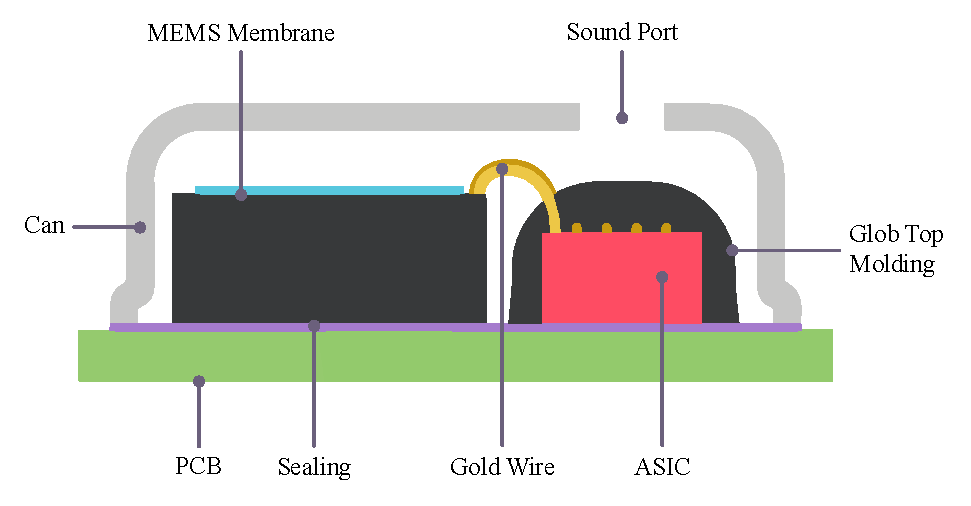
\includegraphics[width=0.9\textwidth]{images/2_preliminaries/mems_microphone_illustration.pdf}
	\caption{Internal structure of a MEMS microphone}
	\label{fig:mems_microphone}
\end{figure}

\subsection{Analog Microphones}
Analog \acrshort{mems} microphones convert sound into an analog electrical signal.
They are simple and easy to integrate in analog circuits but may require additional signal amplification components.
A disadvantage of analog microphones is that they are susceptible to noise and interference, making them unsuitable for long-distance transmission.
\begin{figure}[h!]
	\centering
	\vspace{-0.1cm}
	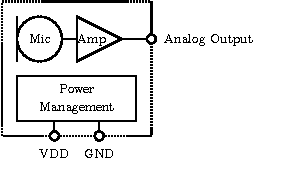
\includegraphics[height=2.9cm, trim={0 0.4cm 0 0}]{images/2_preliminaries/mems_microphone_types_analog.pdf}
	\caption{Block diagram of analog MEMS microphone}
	\label{fig:mems_microphone_types_analog}
\end{figure}

\subsection{PDM Microphones}
\acrshort{pdm} microphones output a digital signal representing the acoustic waveform.
Their digital format is noise-resistant and supports long-distance transmission, making them ideal for multiplexed, multi-microphone setups.
These microphone types require a high-frequency clock signal to operate (typically 1.5\,MHz to 3.25\,MHz),
which must be provided by the host (e.g. a \acrshort{mcu} or \acrshort{fpga}).
A dedicated channel select pin is used to select the microphone's output channel in multiplexed systems.
\begin{figure}[h!]
	\centering
	\vspace{-0.1cm}
	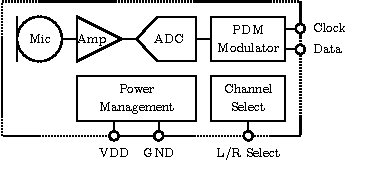
\includegraphics[height=2.9cm, trim={0 0.4cm 0 0}]{images/2_preliminaries/mems_microphone_types_pdm.pdf}
	\caption{Block diagram of PDM MEMS microphone}
	\label{fig:mems_microphone_types_pdm}
\end{figure}

\subsection{PCM Microphones}
\acrshort{pcm} microphones provide a digital output using the \acrlong{pcm} format, most often interfaced via the \acrshort{i2s} protocol.
Compared to \acrshort{pdm} microphones, \acrshort{pcm} microphones have a build-in decimation filter, which simplifies the signal processing chain, as the host no longer needs to perform this task.
However, \acrshort{pcm} microphones are more complex, costly and less common in the industry than \acrshort{pdm} microphones.
\begin{figure}[h!]
	\centering
	\vspace{-0.1cm}
	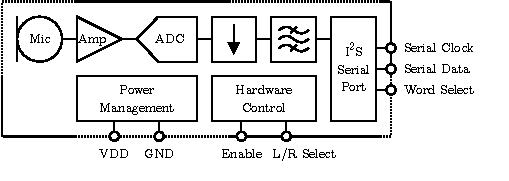
\includegraphics[height=2.9cm, trim={0 0.4cm 0 0}]{images/2_preliminaries/mems_microphone_types_pcm.pdf}
	\caption{Block diagram of PCM MEMS microphone}
	\label{fig:mems_microphone_types_pcm}
\end{figure}
\clearpage

\subsection{Microphone Port Location}
\acrshort{mems} microphones can be categorized based on their port location: top-port and bottom-port.
Top-port microphones have the sound inlet on the top of the package, suitable when the sound source is above the microphone.
Conversely, bottom-port microphones have the inlet at the bottom, ideal for mounting on surfaces where sound comes from the side or below.
For bottom-port microphones, the sound must travel through a hole in the \acrshort{pcb} to reach the microphone, which can affect the sound quality.
\begin{figure}[h!]
	\centering
	\begin{minipage}{0.49\textwidth}
		\centering
		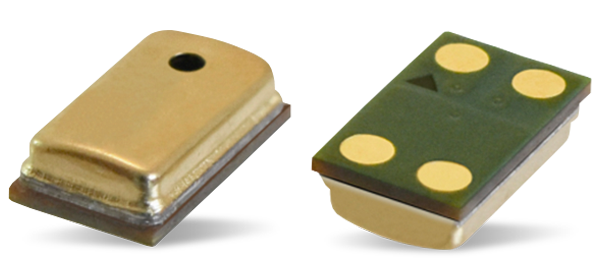
\includegraphics[width=\textwidth]{images/2_preliminaries/mems_microphone_top.png}
		\caption{Top-port MEMS microphone}
		\label{fig:mems_microphone_top}
	\end{minipage}
	\begin{minipage}{0.49\textwidth}
		\centering
		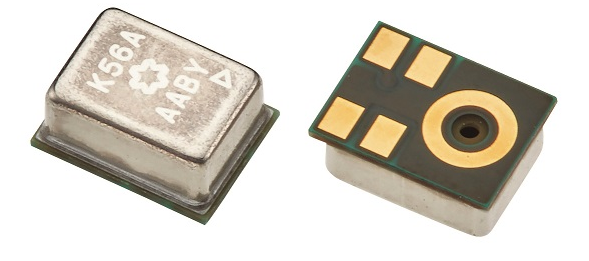
\includegraphics[width=\textwidth]{images/2_preliminaries/mems_microphone_bottom.png}
		\caption{Bottom-port MEMS microphone}
		\label{fig:mems_microphone_bottom}
	\end{minipage}
\end{figure}


\section{Pulse Density Modulation (PDM)}
\acrfull{pdm} is a modulation technique used to represent an analog signal with a binary sequence.
In \acrshort{mems} microphones, the diaphragm movements modulate a high-frequency carrier signal,
resulting in a digital output where the density of pulses corresponds to the amplitude of the input signal.
\acrshort{pdm} simplifies the microphone design, allowing for smaller and more power-efficient devices.
However, it requires a decimation filter in the signal processing chain to convert the high-frequency pulse sequence into a usable digital audio signal.
The \acrshort{pdm} bitstream is encoded from an analog signal through the process of 1-bit delta-sigma (\(\Delta \Sigma\)) modulation.
This process uses a one-bit quantizer that outputs either a 1 or 0 depending on the amplitude of the analog signal.
Due to the nature of real-world analog signals, a quantization error occurs, representing the difference between the 1 or 0 and the actual amplitude it represents.
This error is negatively fed back in the \(\Delta \Sigma\) process loop, influencing every subsequent quantization measurement and its error.
This feedback mechanism averages out the quantization error, enhancing the accuracy of the \acrshort{pdm} representation.
\begin{figure}[h]
	\centering
	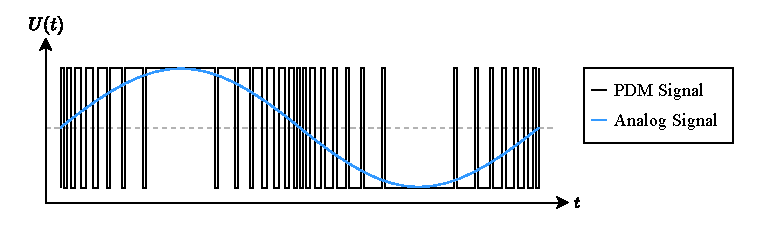
\includegraphics[width=1.0\textwidth]{images/2_preliminaries/pdm_modulation.pdf}
	\caption{PDM Modulation Example}
	\label{fig:pdm_modulation}
\end{figure}


\section{Time Division Multiplexing (TDM)}
\acrfull{tdm} is a method of transmitting and receiving independent signals over a common signal path by means of synchronized switches at each end of the transmission line.
In the context of digital audio, \acrshort{tdm} allows multiple audio streams to share a single communication line,
with each stream getting a dedicated time slot. This technique is valuable in systems where multiple audio channels,
such as in surround sound systems or multi-microphone arrays, need to be transmitted over a single cable.
\acrshort{tdm}'s main advantage is its ability to efficiently handle multiple audio streams without the need for multiple physical connections.
This makes it particularly useful in professional audio applications, broadcast systems, and complex audio setups.
However, \acrshort{tdm} systems can be more complex to implement and require precise synchronization to ensure that the timing of the different channels is maintained.
Figure \ref{fig:tdm_example} shows an example of a TDM-16 system with 16 bits sample width.
\begin{figure}[h]
	\centering
	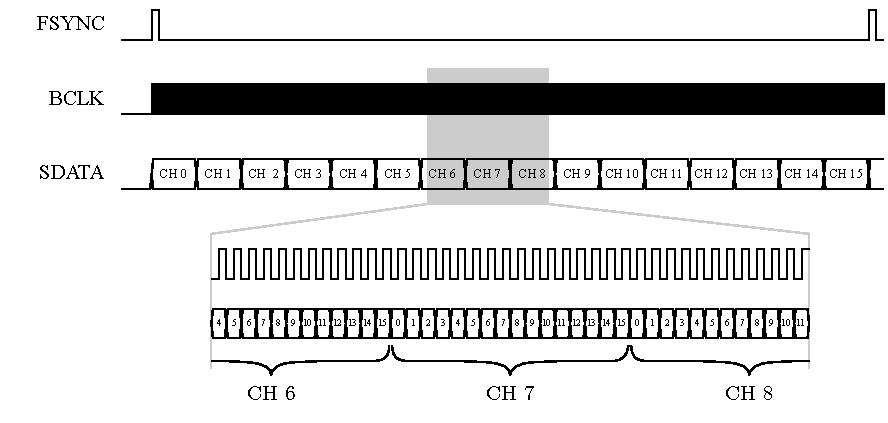
\includegraphics[width=1.0\textwidth, trim={0.5cm 0 0 0}]{images/2_preliminaries/tdm_signals.pdf}
	\caption{Example of TDM-16 with 16 bits sample width}
	\label{fig:tdm_example}
\end{figure}

\acrfull{tdm} systems introduces tristate outputs, enabling multiple devices to share the same physical bus without interference.
The \acrshort{tdm} bus consists of three signals: \textit{fsync}, \textit{bclk} and \textit{data}.
\begin{itemize}
	\item \textbf{FSYNC (Frame Sync)}: This signal marks the start of a frame in the TDM stream.
	      It acts as a reference point for aligning the data across all channels.
	      In a TDM-16 system, FSYNC indicates the beginning of a sequence of 16 channels (slots).
	\item \textbf{BCLK (Bit Clock)}: This clock signal dictates the timing for data transmission.
	      Each edge of the BCLK corresponds to a bit position in the data stream.
	      For 16-bit samples, there are 16 BCLK pulses per channel, hence 256 BCLK pulses per frame.
	\item \textbf{Data}: The actual audio data is transmitted in a series of bits.
	      In a 16-channel, 16-bit TDM system, each channel's data is represented by 16 bits (Left Justified).
\end{itemize}


\section{GNSS Real-Time Kinematic (RTK)}
The \acrfull{gnss} \acrfull{rtk} is an advanced technique used in geodesy and navigation
that enhances the precision of position data derived from satellite-based positioning systems.
\acrshort{rtk} uses differential techniques to improve the accuracy of position information obtained from satellite systems like
\acrshort{gps}, GLONASS, Galileo, or BeiDou.
This method is particularly useful in applications requiring high precision,
such as surveying, construction, and precision agriculture.

\subsection{Custom Node as an Anchor}
One method to utilize \acrshort{rtk} for achieving enhanced position accuracy involves using a custom node as an anchor.
This method requires setting up a fixed \acrshort{rtk} base station at a known location.
The base station calculates error values for satellite signals by comparing the expected signal (based on its known location) with the received signal.
These error values, which account for various factors like atmospheric interference and satellite orbit errors,
are then transmitted to a mobile \acrshort{rtk} receiver.
The mobile receiver uses these corrections to adjust its own satellite signal measurements, significantly improving its positional accuracy.

\subsection{Using Data from a Public Provider}
Alternatively, \acrshort{rtk} corrections can be obtained from a public provider.
In this approach, the user does not set up a custom anchor node but instead subscribes to a service that provides \acrshort{rtk} correction data.
These services operate a network of \acrshort{rtk} base stations and compute correction factors for different regions.
The correction data is typically transmitted via the internet directly to the user's \acrshort{rtk} receiver.
This method is convenient for users who do not have the resources to establish and maintain their own \acrshort{rtk} base station.
By applying these corrections, which include compensating for atmospheric drift and other errors,
the user's receiver can achieve a similar level of enhanced positional accuracy as with a custom anchor node.

\graphicspath{ {images/3_source_localization/} }
\chapter{Sound Source Localization}
\section{Physical background}
This section shows some underling fundamentals on which the following described theory is based on.
\todo{Schribe}

\section{Sound Source Localization Methods}
\acrfull{ssl} is a well researched area with many applications.
\cite{nat_skript}
The basic system can be brought into two categories, time based or power based methods.
\subsection{Power based SSL}
The idea of power based SSL is based of the known propagation properties of sound waves in air.
BlaBlaBla \todo{short text}
However for this method to work some properties of the sound source have to be known.
Additionally the sensors that measure the sound power levels have to be calibrated \dots

\subsection{Time Based SSL}
Another group of \acrshort*{ssl} is based on the time when the
signal is received by the microphones.
Given a source at a location $\bm{S} = (x_S,y_S)^T$ and $N$ microphones at locations
$\bm{M_n} = (x_n,y_n)^T$ the time it takes for a acoustic signal from the source to reach a microphone is
\begin{equation}
	t_n = \frac{\lVert \bm{S} - \bm{M_n}\rVert}{c}
	= \frac{\sqrt{\left(x_S - x_n\right) + \left(y_S - y_n\right)}}{c} .
\end{equation}
So if $t_n$ is known for a microphone, the location of the source can be limited to point on a circle
around $M_n$ with a radius of $t_n c$.
Given three or more microphones the intersection of these circles will show th location of the source.
However in many cases this approach is not realistic since $t_n$ is generally not know.
It would require some sort of a synchronization between the microphones and the sources.
\subsubsection{Near-Field}
The next time property that could be used is the \acrfull{tdoa} which between
two microphones $\bm{M_n}$ and $\bm{M_m}$ is defined as
\begin{equation}
	t_{n, m} = t_m - t_n = \frac{\lVert \bm{S} - \bm{M_m}\rVert - \lVert \bm{S} - \bm{M_n}\rVert}{c}.
\end{equation}
With this equation $\bm{S}$ can be interpreted as the set of points that lie on a hyperbola
which fixed points are the Microphones and the vertices are $c t_{n,m}$m apart.
To find the location of $\bm{S}$ a minimum of four microphones is now needed.
This approach works only if we can assume that the curvature of the incoming sound waves
at the microphones is big enough. Figure \ref{ssl:fig:near field} shows such a arrangement
which is generally known as the near-field scenario.
It is generally said, that the near-field assumption holds when the distance from the source
to the array isn't much greater than the size of the array.
In Figure \ref{ssl:fig:hyperbola} it can be seen how the resulting hyperbolas from the
\acrshort{tdoa} intersect at the point $\bm{S}$.


\begin{figure}[h]
	\centering
	\begin{subfigure}[b]{0.45\textwidth}
		\centering
		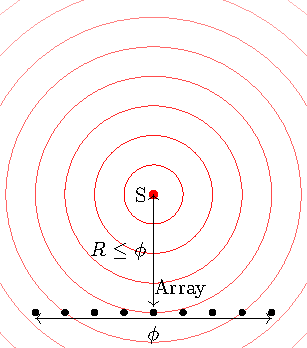
\includegraphics[width=\textwidth]{NearField.pdf}
		\caption{Acoustic model used for the near field \acrshort{ssl}.}
		\label{ssl:fig:near field}
	\end{subfigure}
	\hfill
	\begin{subfigure}[b]{0.45\textwidth}
		\centering
		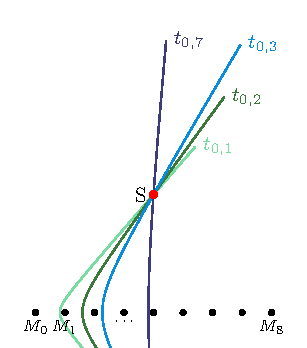
\includegraphics[width=\textwidth]{hyperbola.pdf}
		\caption{A selection of the hyperbolas resulting from the time-delays $t_{m,n}$.}
		\label{ssl:fig:hyperbola}
	\end{subfigure}
	\caption{Near field \acrshort{ssl} with a linear microphone Array.
		Since the microphones are distributed on a straight line a degree of freedom is lost and
		$\bm{S}$ mirrored at this line is also a possible solution.}
	\label{fig:three graphs}
\end{figure}

\subsubsection{Far-Field}
When the source is much further away than the size of the Array, as depicted
in Figure \ref{ssl:fig:far field}, the curvature of the sound wave at the array is negligible.
This is generally known as the far-field case.
Now the sound waves aren't modeled as spherical waves but rather as planar waves.
Given such a planar wave only the direction in which the source is placed can be determined with the TDOAs.

% Beamforming_general_S1110865703212038

\begin{figure}
	\centering
	%    \includegraphics[width=0.25\textwidth]{mesh}
	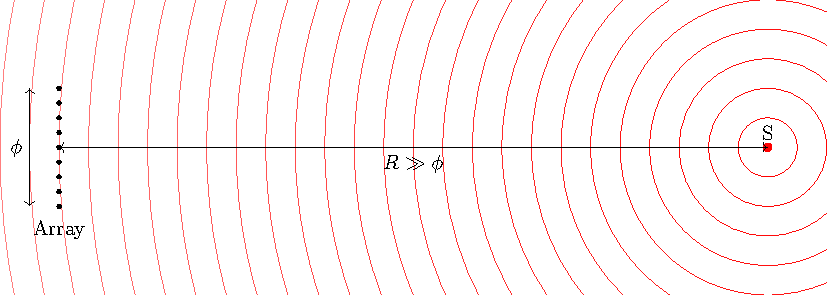
\includegraphics[]{FarField.pdf}
	\caption{Far-Field case. The Curvature of the sound-waves from S at the array
		is almost zero.}
	\label{ssl:fig:far field}
\end{figure}

\todo{Decission why this}
In this thesis the focus is set on the far-field case, due
\todo{literature}

\subsection{Direction of arrival estimation}
Lots of research has been made on how to estimate the \acrfull*{doa} of a source
with appropriate sensors.

\todo{brief lierature study}

In this thesis the focus was set on far-field techniques considering that the
goal is to detect drones which are usually several meters above ground.
%Constructing a microphone array 

\subsection{Beamforming}
Beamforming is a popular method for estimating the \acrshort{doa} of a signal.

To better show the fundamental principles of beamforming an example is used
where the goal isn't to estimate a \acrshort{doa} but to send a signal
in a desired direction using microphones.
Figure \ref{ssl:fig:beamforming1} shows such a case in $\mathbb{R}^2$
where a linear array of N sound sources beam a sine wave $x(t) = \sin(\omega_0 t)$ 
in the direction of $\varphi$.
This is achieved by adding a phase shift to the sine wave
at each microphone resulting in $x_n(t) = sin(\omega_0 t + \omega_0t_n)$.
When the phase shifts are properly selected the points where the waves positively
interfere form a beam.
Given this example with a narrow band signal, the signal at each source
can be written as
\begin{equation}
	x_n(t) = \Re(sin(\omega_0 t) e^{j\omega t_n})
\end{equation}
and more generalized as 
\begin{equation}
  \label{ssl:eq:beamSteerOut}
  X(t, \varphi) = 
  \Re\left(
    sin(\omega_0 t)
    \underbrace{
      \begin{pmatrix} 
        e^{-j\omega_0 t_0(\varphi)} \\ 
        e^{-j\omega_0 t_1(\varphi)} \\
        \vdots \\ 
        e^{-j\omega_0 t_{N-1}(\varphi)} 
      \end{pmatrix}}_{W(\varphi)}
  \right).
\end{equation}
The vector $W(\varphi)$ is commonly known as the steering vector.
It can be seen that the steering vector is dependent on $\omega_0$ and 
will therefore only have the desired effect on signals with frequencies 
close to $\omega_0$.
How to use beamforming with wider band signals will be shown later in this chapter.
\begin{figure}
	\centering
	%    \includegraphics[width=0.25\textwidth]{mesh}
	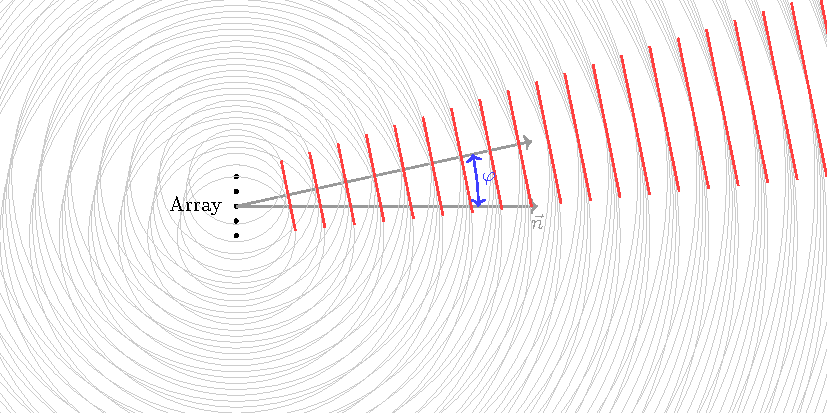
\includegraphics[]{beamforming_1.pdf}
	\caption{Phase differences between the array elements create positive interference at the red lines.
		The gray circles correspond the waves' local maxima}
	\label{ssl:fig:beamforming1}
\end{figure}

If the goal is to estimate the direction of a sound signal with microphones 
$x_n(t)$ is now defined as the signal measured by the nth microphone.
Now \eqref{ssl:eq:beamSteerOut} is rewritten to 
\begin{equation}
  \label{ssl:eq:beamSteerIn}
  \bm{Y(t, \varphi)} = 
    \underbrace{
      \begin{pmatrix} 
        x_0(t) \\ 
        x_1(t) \\
        \vdots \\ 
        x_{N-1}(t)
    \end{pmatrix}}_{X(t)}
    \odot
    \underbrace{
      \begin{pmatrix} 
        e^{-j\omega_0 t_0(\varphi)} \\ 
        e^{-j\omega_0 t_1(\varphi)} \\
        \vdots \\ 
        e^{-j\omega_0 t_{N-1}(\varphi)} 
      \end{pmatrix}}_{W(\varphi)}
\end{equation}
where depending on the method used either $Y(t, \varphi)$ is further processed, or the 
method directly uses $X(t)$ for the \acrshort*{doa} estimation.

\subsubsection{Steering Vector}
The calculation of the Steering Vector is dependent on different factors.
The two main factor can be broken down to the geometry of the microphone array
and the direction in which the source lies. 
Again the formulas are derived for a circular array in $\mathbb{R}^2$ and are then expanded into $\mathbb{R}^3$.
A circular array where all the microphones are 
placed on a circle is convenient for the use of polar coordinates and the 
formulas can also be used for any other array described in polar coordinates.

Figure \ref*{ssl:fig:steering} shows such an array with five equally spaced microphones $M_n$.
The goal of the steering vector is to delay the measured signal at each microphone so that
they each have the same phase and therefore positively interfere.
To calculate these delays a reference point must firstly be defined, here it is the center of the circle.
Because a far-field model is used the sound pressure level is equal along lines perpendicular
to its propagation direction.
With the magenta line as the reference line, each measured signal from the microphones must be
phase shifted with 
\begin{equation}
  \omega_0 t_n = 
  \omega_0 \frac{
    \lVert\bm{d}_n(\varphi_s)\rVert}
    {c} 
    \hat{\bm{d}}_n(\varphi_s) \cdot \hat{\bm{d}}_s.
\end{equation}
The Term $\hat{\bm{d}}_n(\varphi_s) \cdot \hat{\bm{d}}_s$ is needed to determine
if a phase shift is positive or negative.
Using the trigonometric properties of a right triangle
\begin{equation}
  \lVert\bm{d}_n(\varphi_s)\rVert \hat{\bm{d}}_n(\varphi_s) \cdot \hat{\bm{d}}_s = r_{m_n} \cos(\varphi_s - \varphi_{m_n})
\end{equation}
and therefore
\begin{equation}
  t_n = 
  r_{m_n} \cos(\varphi_s - \varphi_{m_n})
  \frac{1}{c}.
  \label{ssl:eq:beamr2}
\end{equation}
This formula can be used for any microphone with polar coordinates
$(\varphi_{m_n}, r_{m_n})$ and can therefore be used for any array configuration
described in polar coordinates.
\begin{figure}
  \centering
  %    \includegraphics[width=0.25\textwidth]{mesh}
  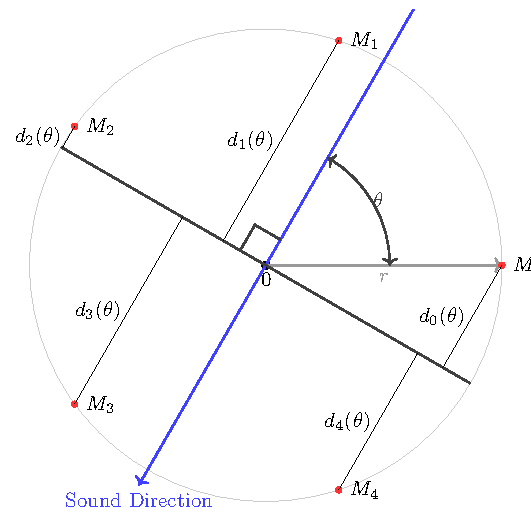
\includegraphics[]{steering_vector.pdf}
  \caption{BalaBula}
  \label{ssl:fig:steering}
\end{figure}

To expand this idea into $\mathbb{R}^3$ the spherical coordinate system is now used.
This adds the angle $\theta$ as the inclination.
When $\theta = \pi/2$ it is the same situation that has already been looked at.
But as $\theta$ aproaches 0 the speed of the wavefront projectet onto the
surface of the array increases. 
This adds a term to \eqref{ssl:eq:beamr2}
\begin{equation}
	t_n = 
	r_{m_n} \cos(\varphi_s - \varphi_{m_n})
	\frac{\omega \sin(\theta)}{c}.
  \label{ssl:eq:beamr3}
\end{equation}

\subsubsection{Delay and Sum Beamformer}
The basic beamformer is the delay and sum Beamformer
\begin{equation}
	\label{ssl:eq:delAndSum}
	y(t, \varphi, \theta) = 
	  \underbrace{
		\begin{pmatrix} 
		  x_0(t) \\ 
		  x_1(t) \\
		  \vdots \\ 
		  x_{N-1}(t)
	  \end{pmatrix}}_{X(t)}
	  \cdot
	  \underbrace{
		\begin{pmatrix} 
			e^{-j\omega_0 t_0(\varphi, \theta)} \\ 
			e^{-j\omega_0 t_1(\varphi, \theta)} \\
			\vdots \\ 
			e^{-j\omega_0 t_{N-1}(\varphi, \theta)} 
		\end{pmatrix}}_{W(\varphi, \theta)}.
\end{equation}
Notice how intead of the Hadamard product, the scalar product is now used.
$y(t, \varphi, \theta)$ is therefor the sum of the delayed signals.
If the angles of the steering vector point towards a source its 
signal will be amplified.
By using the delays calculated for the steering vector $X(t)$ can
be calculated to simulate a source in a specifig direction
\begin{equation}
	X(t, \varphi_s, \theta_s) = 
	e^{j\omega_0 t}
	\begin{pmatrix} 
		e^{j\omega_0 t_0(\varphi_s, \theta_s)} \\ 
		e^{j\omega_0 t_1(\varphi_s, \theta_s)} \\
		\vdots \\ 
		e^{j\omega_0 t_{N-1}(\varphi_s, \theta_s)} 
	\end{pmatrix}
\end{equation}
The amplitude response of an array using delay and sum beamforming can
now be calculated with
\begin{equation}
	G(\phi, \theta) = 
	\frac{
		\lvert X(0, \phi_s, \theta_s) \cdot W(\phi, \theta) \rvert}
	{
		N
	}.
\end{equation}
The response is normalized with the ammount of microphones to ensure a maximum
gain of 1.
In Figure \ref*{ssl:fig:CircBmResponse} two such repsonses with can be seen.
The main lobe of $G(\phi, \theta)$ clearly shows in the direction of the source
however there are also side lobes pointing to directions whithout sources.
How they behave is later discussed in \todo{chapter reference}.

\begin{figure}[h]
	\centering
	\begin{subfigure}[t]{0.45\textwidth}
		\centering
		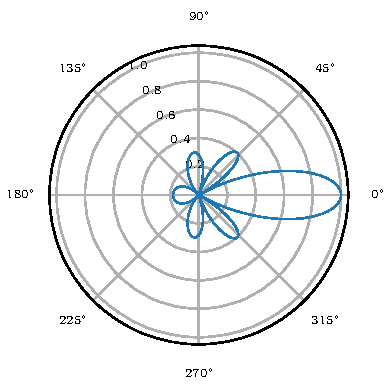
\includegraphics[width=\textwidth]{radial_1200_circ_single.pdf}
		\caption{\(G(\phi, \theta, \omega)\) with $\theta = \pi/2$ for $\omega_0 = 2\pi 1000$.
		The source is placed in the direction of $(\phi=0, \theta = \pi/2)$}
		\label{ssl:fig:CircBmPhi}
	\end{subfigure}
	\hfill
	\begin{subfigure}[t]{0.45\textwidth}
		\centering
		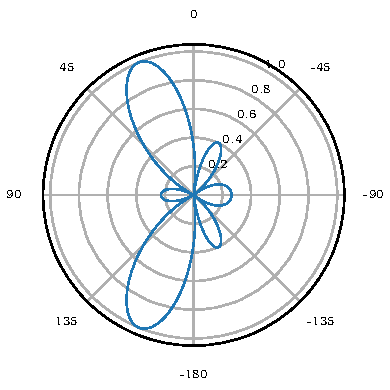
\includegraphics[width=\textwidth]{radial_1200_circ_theta_single.pdf}
		\caption{\(G(\phi, \theta, \omega)\) with $\phi = 0$ for for $\omega_0 = 2\pi 1000$. 
		$(\phi= 0, \theta = -45^\circ)$ is the same as $(\phi= 180^\circ, \theta = 45^\circ)$.
		The mirror along the horizontal axis comes from the flat geometry of the array which makes
		it impossible to distinguish if a sound comes from $\theta$ or $180 + \theta$.} 
		\label{ssl:fig:CircBmTheta}
	\end{subfigure}
	\caption{Delay and Sum Beamformer response for a circular array with $N=16$ microphones 
	and a radius $r = 0.25$m. }
	\label{ssl:fig:CircBmResponse}
\end{figure}

Until now the formulas are only useful for narrow band signals. 
This theroy is now expanded to be applicable for wide band signals.
The narrow band delay and sum beamformer has the property, that it behaves
the same in the freqeuncy domain
\begin{equation}
	e^{-j\omega_0 t_n} x_n(t) = \mathscr{F}^{-1}(e^{-j\omega_0 t_n} \mathscr{F}(x_n(t)))
\end{equation}
since it's just a multiplication with a scalar,. 
The summation could also be done in the frequency domain due to the 
linearity of the Fourier transform.
However in the frequency domain a IIR Filter can be consructed, to 
make a different phaseshift for every frequency 
\begin{equation}
	\label[type]{ssl:eq:iirbeam1}
	Y_n(t) = \mathscr{F}^{-1}(e^{-j\omega t_n} X_n(\omega)).
\end{equation}
By using a discrete fourier transform the beamformer can be written
in matrix form
\todo{Indexchaos lösen}
\begin{equation}
	Y(\omega, \phi, \theta) = 
	\begin{pmatrix}
		X_0(\omega_l) & \hdots & X_0(\omega_h)\\
		\vdots & \ddots & \vdots \\
		X_{N-1}(\omega_l) & \hdots & X_{N-1}(\omega_h)
	\end{pmatrix}^T
	\odot
	\begin{pmatrix}
		e^{-j\omega_l t_0} & \hdots & e^{-j\omega_h t_0}\\
		\vdots & \ddots & \vdots \\
		e^{-j\omega_l t_{N-1}} & \hdots & e^{-j\omega_h t_{N-1}}
	\end{pmatrix}^T.
\end{equation}
\subsection{Other beamforming techniques}
\newpage
\section{Simulator}
In order to experiment with different microphone arrangements and algorithms a simulator was developed.
Since the simulator wasn't the main focus of this Thesis, its functionality was kept simple.
The simulator lets you place acoustic sources and microphones in a $\mathbb{R}^3$ space and calculates
the measured signals at each microphone.

\subsection{Simulation Model}
For sake of simplicity the sources were modeled as omnidirectional point-sources and the
microphones are omnidirectional as well.
The Sound Pressure Level of a source is defined at one meter distance from their position and decreases
squarely with the distance.
The perceived sound at any point $P$ can now be described as
\begin{equation}
	\label[type]{ssl:eq:simcont}
	y(P, t) = \sum_{I} \frac{x_i(t - \lVert P - S_i\rVert/c)}{\lVert P - S_i\rVert}.
\end{equation}
Where $S_i$ is the position of the nth Source and $x_i(t)$ is its output sound.
Since the simulation is done numerically and with pre recorded audio files with a given
samplingrate $f_s$ \eqref{ssl:eq:simcont} has to be discretized.
Simply replacing $x_i(t - \lVert P - S_i\rVert/c)$ with
$x_i(n - f_s \lVert P - S_i\rVert/c)$ with
$n \in \mathbb{N}$ doesn't work because
$f_s \lVert P - S_i\rVert/c \not \in \mathbb{N}$ in most cases.
To implement this $f_s \lVert P - S_i\rVert/c$ is rounded to
its nearest integer $d_{P,S_i}$.
Now the delayed signal is $x_i(n - d_{P,S_i})$.
To achieve sub sample delays this signal is then filtered
with a Fractional Delay FIR Filter with a delay of
$f_s \lVert P - S_i\rVert/c - d_{P,S_i}$.

\subsubsection{Reflections}
The simulator also allows the reflective surfaces to be placed into the room.
These surfaces are defined with \todo{wiauimeer} and have a infintie size.
Additionally a dampening factor can be defined which defines how much 
a reflecting sound signal is damped when getting reflected.
By this stage the simulator can only handle single reflective path. 
An already reflected sound signal can not be reflected by a second surface.



\chapter{Acquisition-System Design}
\section{Overview}
This section covers the development process including the hardware and firmware design of the audio acquisition system.
The goal of the acquisition system is to provide a flexible microphone recording infrastructure to easily aquiring audio signals from multiple microphones.


\subsection{Key Requirements}
% The main focus of the development is to design a professional looking, easy to use and eye-catching device for demonstration purposes.
% The project name \textit{Audio-Beamformer} has been chosen as it is easy to remember and has potential to be seen as a trademark.

The following key requirements have been set:
% \begin{itemize}
% 	\item Single power adapter or power cable (e.g. no need of labor power supplies)
% 	\item Easy to install (e.g. montage on a camera tripod)
% 	\item Intuitive to operate via state-of-the-art graphical user interface
% 	\item Multiple audio streaming sources such as Bluetooth and USB input devices
% 	\item Great scalability and flexibility of the hardware and software design
% \end{itemize}

\subsection{Key Decisions}



\newpage
\section{Hardware Design}

\begin{figure}[h]
	\centering
	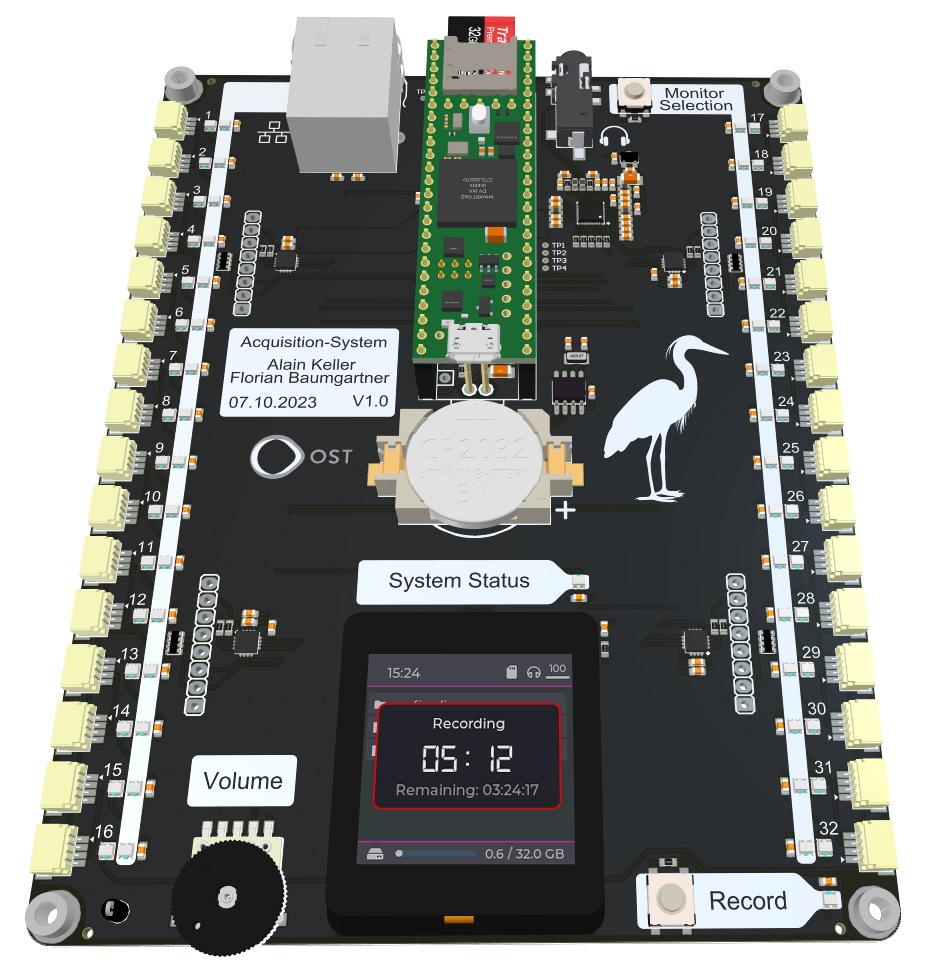
\includegraphics[width=1.0\textwidth]{images/4_design_acquisition_system/Acquisition_System_Front.png}
	\caption{Front view of the Acquisition System}
	\label{fig:acquisition_system_front}
\end{figure}


\subsection{Block Diagram}

\begin{figure}[h]
	\centering
	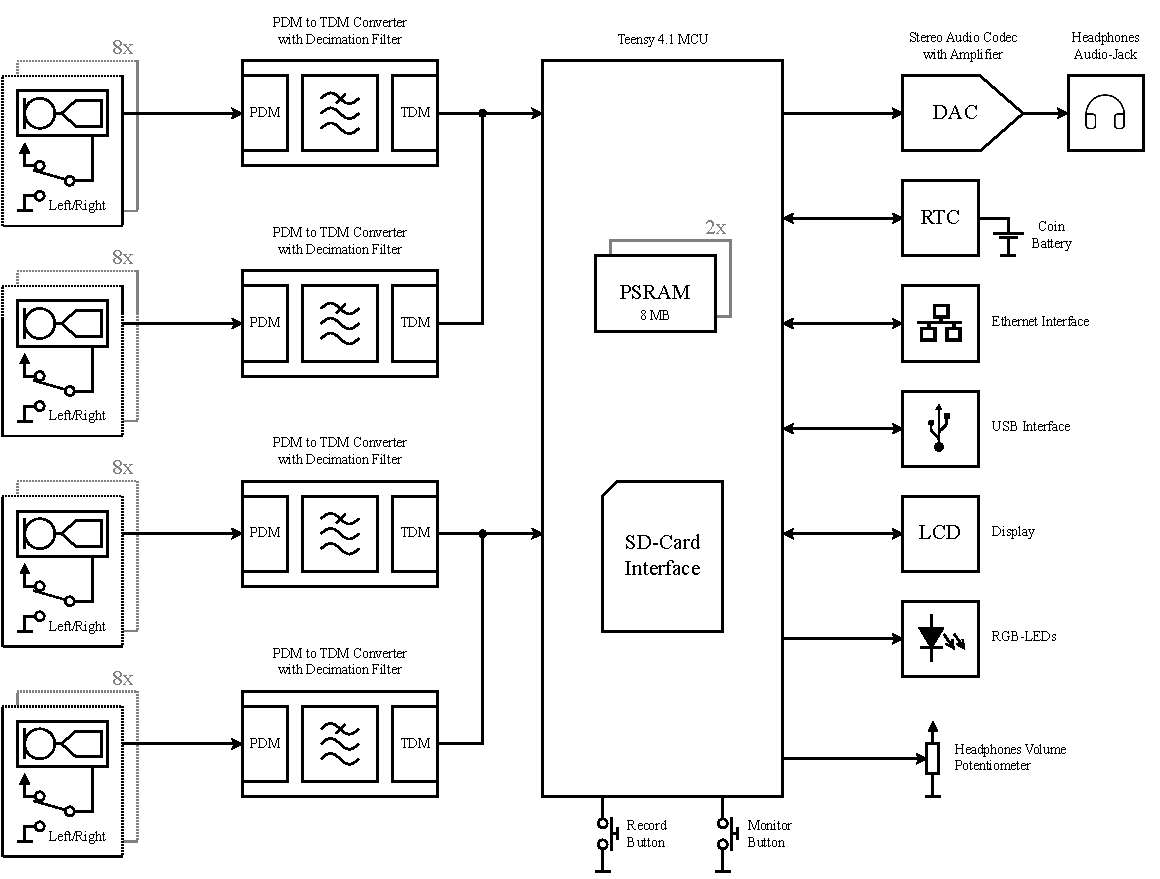
\includegraphics[width=1.0\textwidth]{images/4_design_acquisition_system/system_block_diagram.pdf}
	\caption{System block diagram}
	\label{fig:system_block_diagram}
\end{figure}

\subsection{Microcontroller Unit (MCU)}

%  TODO: Write about external PSRAM


\subsection{Audio Input}

\subsection{Audio Processing}

\subsection{Headphone Output}

To prelisten the individual audio channels, a headphone output is implemented.

% description of headphones jack
The headphone output is a standard 3.5mm stereo jack.



\newpage
\section{Firmware Design}
Blabla

\subsection{Graphical User Interface (GUI)}

\subsection{GUI Pages}

\begin{minipage}{\linewidth}
	\begin{wrapfigure}{l}{4.5cm}
		\vspace{-0.6cm}
		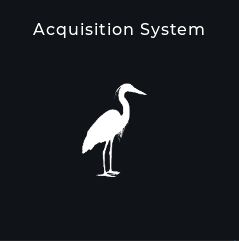
\includegraphics[width=4cm]{images/4_design_acquisition_system/gui/01_splash_screen.png}
		\centering
		\caption{Splash screen}
		\label{fig:acquisition_system_gui_splash_screen}
	\end{wrapfigure}
	\subsubsection{Splash Screen}
	When the device is powered on, the splash screen is displayed until the boot process is finished.
	On average this takes about 5 seconds.
\end{minipage}
\vspace{-0.2cm}




\chapter{Array Evaluation}
\section{Overview}
As stated in chapter \dots the geometry of a microphone array
has a impact on the performance of beamforming.
The goal is to find a well suited array geometry for the detection and tracking of
Drones.
To achieve this, first some array geometries have been simulated and then
a prototype was built to gather information on how they perform in reality.
Then the real data were compared to the simulated data to
confirm the validity of the simulation.
In the next step the findings of the prototypes and simulations
were used to come up with a final array design.

By analysing the sound of some commercially available drones
a desired frequency range of 500 to 2000 hz was set.
This range includes most of the sound's energy.

The array geometry has some contraints, 
such as the number of microphones and the mechanical feasibilty.
As stated in \ref*{chap:AqqSys} the maximum number of microphones
in an array is 32.

To compare different array geometries, several simulations
were ran for each array.
The simulated data was then ran through the beamforming 
algorithm.
The steering angles are based on a grid with $-180^\circ \leq \phi < 180\circ$ and 
$0^\circ \leq \theta \leq 180^\circ$ with a spacing of $1^\circ$.
For each point in this grid the power over the desired frequency band is calculated.
Displaying the result leads to an image like Figure \ref*{aev:fig:gridEx}.
The visualizations may be misleading depending on the angle.
This is a result from the projection of the semisphere onto a 2-d surface.
\begin{figure}
	\centering
	%    \includegraphics[width=0.25\textwidth]{mesh}
	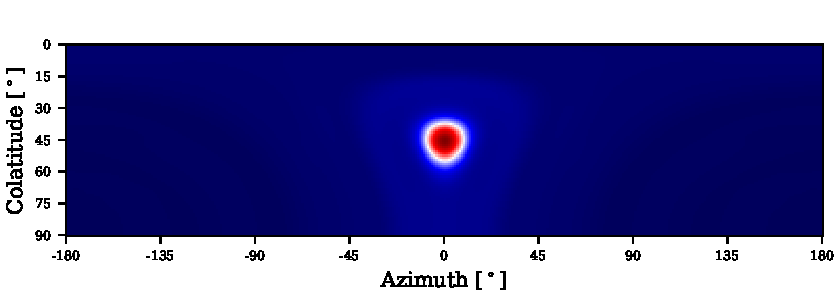
\includegraphics[]{images/5_array_evaluation/0.5_0.79.pdf}
	\caption{PGurke}
	\label{aev:fig:gridEx}
\end{figure}
\section{Metrics}
TO evaluate the performance of an array several metrics are used.
In \todo{Cite Array design s40430-018-1275-5-1, array design comparisons} the
main beam-width is proposed.
\todo{cite Circ array drone trackings13638-019-1632-9} is using the ratio
between the main lobe power and the side lobe power.
Another measure related to the main lobe with is the main lobe area.s
The main lobe is defined as all the points around the peak where their value
is greater than half the peaks value. \todo{besser englisch}

\subsection{Area}
Since the grid resulting from the beamforming represents spherical function
simply taking the sum of all the gridpoints from the mainlobe 
would deliver false results. 
So each grid point is normalized by the surface element of a sphere
\begin{equation}
	dA = r \sin\theta \, d\phi \cdot r d\theta.
\end{equation}
The area of the mainlobe determines how good different sources can be separated.
With a big mainlobe area two close sources may lead to one bigger mainlobe instead
of two seperable ones.
\subsection{Peak Average Power ratio}
The Peak Average Power ratio is the ratio between the peak power and
the average power over the whole grid.
The results from the projection are compenstatet by weighting
the power at each grid cell with the area of that grid cell. 


Blabla
\section{Array Geometry}
In \todo{cite} the authors use a circular array to detect and track drones.
They however did not gave any reasoning no why the chose a circular array.
\cite{bandkProducts}
In \cite{arr1} different array types are compared and measured.
The best scores are reached with the Underbrink style array, a combination
of multiple circular arrays.
They also included several spiral based arrays
Based on this three main groups of arrays were further analysed,
the circualr array, an adaption of the underbrink array, and a archimedes
spiral array.
\subsection{Circular Array}
The circular array is the most simple shape of these three.
It has two degrees of freedom, the circle radius and the number of microphones.
Figure \ref*{aev:fig:MicCirc} shows how the PAP ratio changes when
more microphones are added to an array with a fixed radius.
For smaller array the best PAP they can have is reached with less
microphones than the bigger ones need.
\dots Hallo Satz
The radius of the array has a big impact on how the lower frequencies
smear out the peak.


\begin{figure}
	\centering
	%    \includegraphics[width=0.25\textwidth]{mesh}
	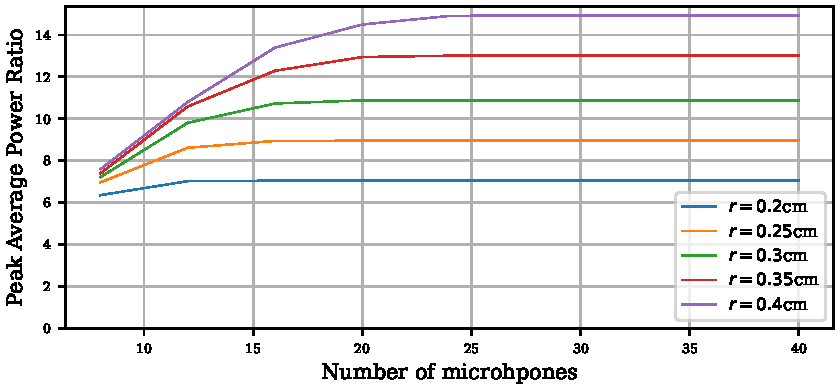
\includegraphics[]{images/5_array_evaluation/circ_m_pap.pdf}
	\caption{PAP ratio for different array radiuses and total number
	of microphones.}
	\label{aev:fig:MicCirc}
\end{figure}
\begin{figure}
	\centering
	%    \includegraphics[width=0.25\textwidth]{mesh}
	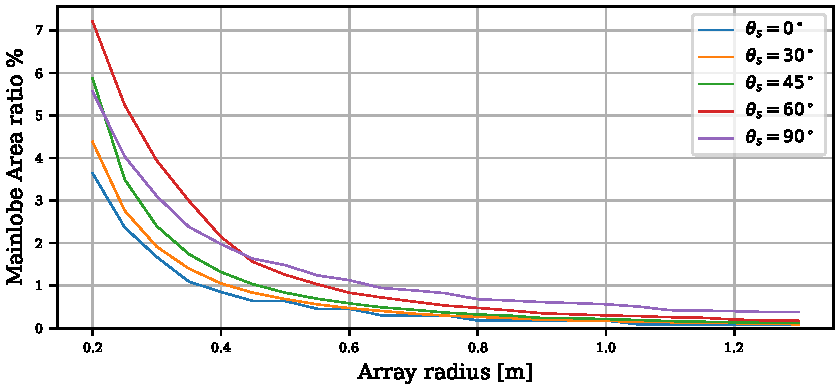
\includegraphics[]{images/5_array_evaluation/area_circ.pdf}
	\caption{Ratio of the mainlobe area compared to the area of a half sphere for 
	a circular array with 32 microphones.}
	\label{aev:fig:areaCirc}
\end{figure}
\begin{figure}
	\centering
	%    \includegraphics[width=0.25\textwidth]{mesh}
	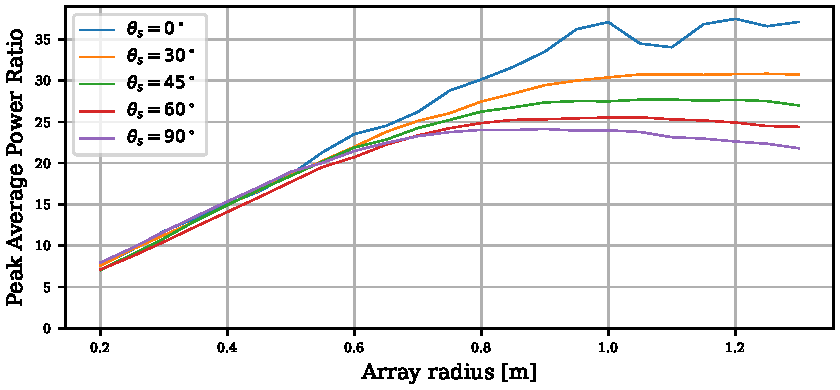
\includegraphics[]{images/5_array_evaluation/PAP_circ.pdf}
	\caption{Peak Average }
	\label{aev:fig:papCirc}
\end{figure}
\dots
\subsection{Underbrink Array}
\dots
\subsection{Archimedes Spiral Array}

\newpage
\section{Mechanical Design}
The mechanical design of the array prototypes was centered around the objective of testing a wide range of array configurations.
To achieve this, two flexible microphone array frames were developed.
A significant aspect of the design process involved determining the overall size of the arrays.
While larger arrays typically offer better performance, practicality and manufacturability had to be considered as well.
In practice, a maximal outer diameter of 60\,cm was chosen for the array prototypes.
Based on simulation results, two specific array types were explored: The Multi-Circular Array and the Archimedean Spiral Array, as described in the next sections.

\subsection{Multi-Circular Array}
\begin{minipage}{\linewidth}
	\begin{wrapfigure}{r}{7.5cm}
		\vspace{-0.8cm}
		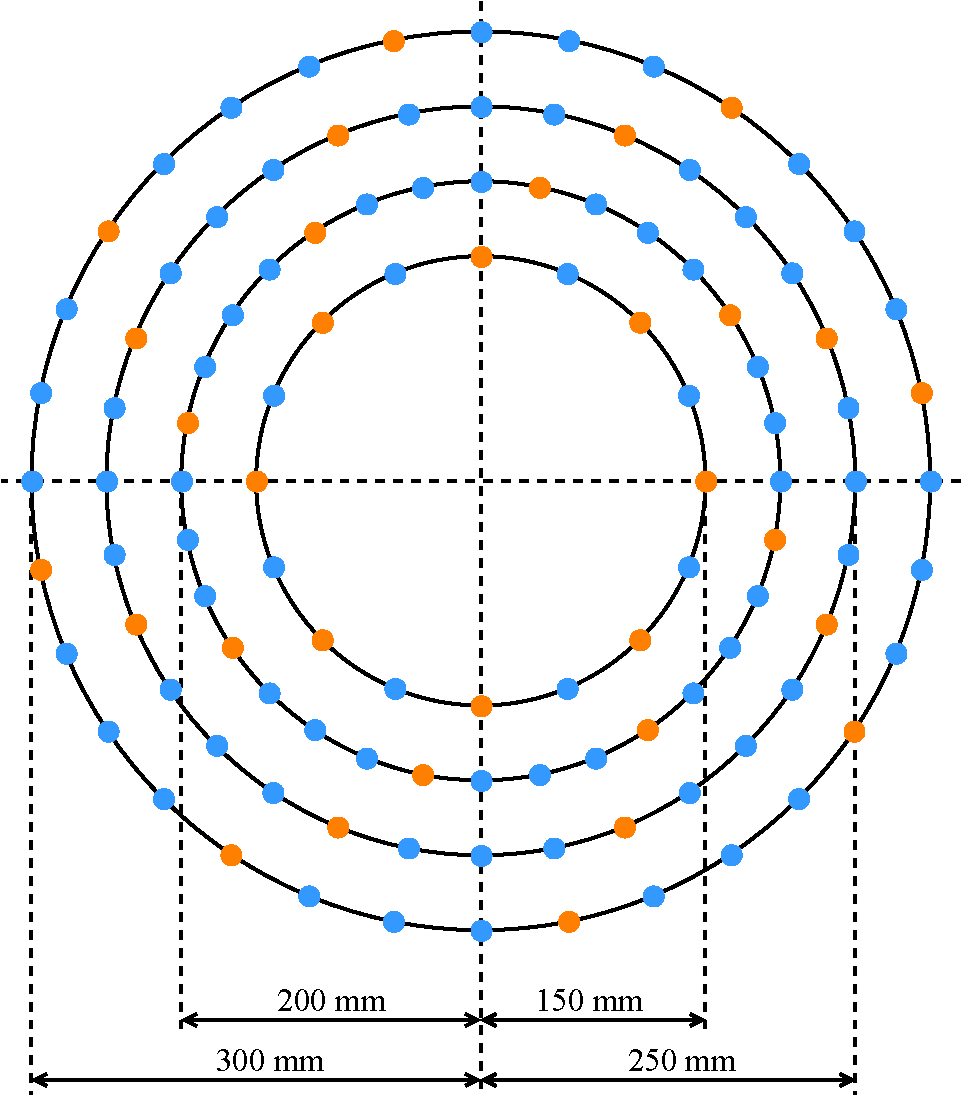
\includegraphics[width=7cm]{images/5_array_evaluation/prototype_array_multi_circular.pdf}
		\centering
		\caption{Multi-Circular Array}
		\label{fig:prototype_array_multi_circular}
	\end{wrapfigure}
	Lorem ipsum dolor sit amet, consetetur sadipscing elitr, sed diam nonumy eirmod tempor invidunt ut labore et dolore magna aliquyam erat, sed diam voluptua.
	At vero eos et accusam et justo duo dolores et ea rebum. Stet clita kasd gubergren, no sea takimata sanctus est Lorem ipsum dolor sit amet.
	Lorem ipsum dolor sit amet, consetetur sadipscing elitr, sed diam nonumy eirmod tempor invidunt ut labore et dolore magna aliquyam erat, sed diam voluptua.
	At vero eos et accusam et justo duo dolores et ea rebum.
	\todo[inline]{\@Alain: Add explanation of the array geometry here}
\end{minipage}
\vspace{0.5cm}    % Adjust this depending on the length of the text above

\subsection{Archimedean Spiral Array}
\begin{minipage}{\linewidth}
	\begin{wrapfigure}{r}{7.5cm}
		\vspace{-0.8cm}
		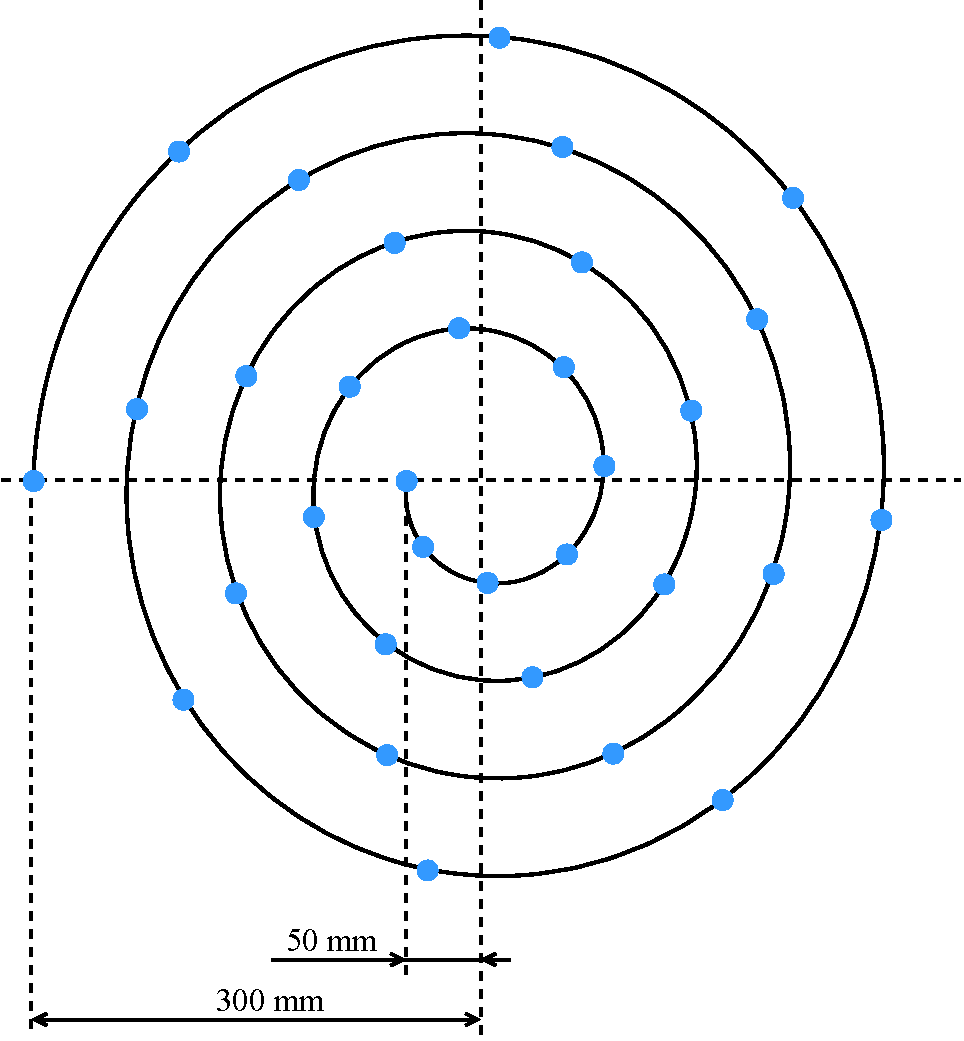
\includegraphics[width=7cm]{images/5_array_evaluation/prototype_array_archimedian_spiral.pdf}
		\centering
		\caption{Archimedean Spiral Array}
		\label{fig:prototype_array_archimedian_spiral}
	\end{wrapfigure}
	Lorem ipsum dolor sit amet, consetetur sadipscing elitr, sed diam nonumy eirmod tempor invidunt ut labore et dolore magna aliquyam erat, sed diam voluptua.
	At vero eos et accusam et justo duo dolores et ea rebum. Stet clita kasd gubergren, no sea takimata sanctus est Lorem ipsum dolor sit amet.
	Lorem ipsum dolor sit amet, consetetur sadipscing elitr, sed diam nonumy eirmod tempor invidunt ut labore et dolore magna aliquyam erat, sed diam voluptua.
	At vero eos et accusam et justo duo dolores et ea rebum.
	\todo[inline]{\@Alain: Add explanation of the array geometry here}
\end{minipage}
\newpage


\subsection{Wooden Prototype Arrays}
Two wooden prototypes, a multi-circular array and an Archimedean spiral array, were manufactured by laser-cutting 5\,mm plywood.
Both arrays had to be split into several pieces due to the limited size of the laser-cutter and were later glued together.
In the centre of each array, a mechanical mount for the Acquisition-System hardware was integrated.
\begin{figure}[h!]
	\centering
	\begin{minipage}{0.49\textwidth}
		\centering
		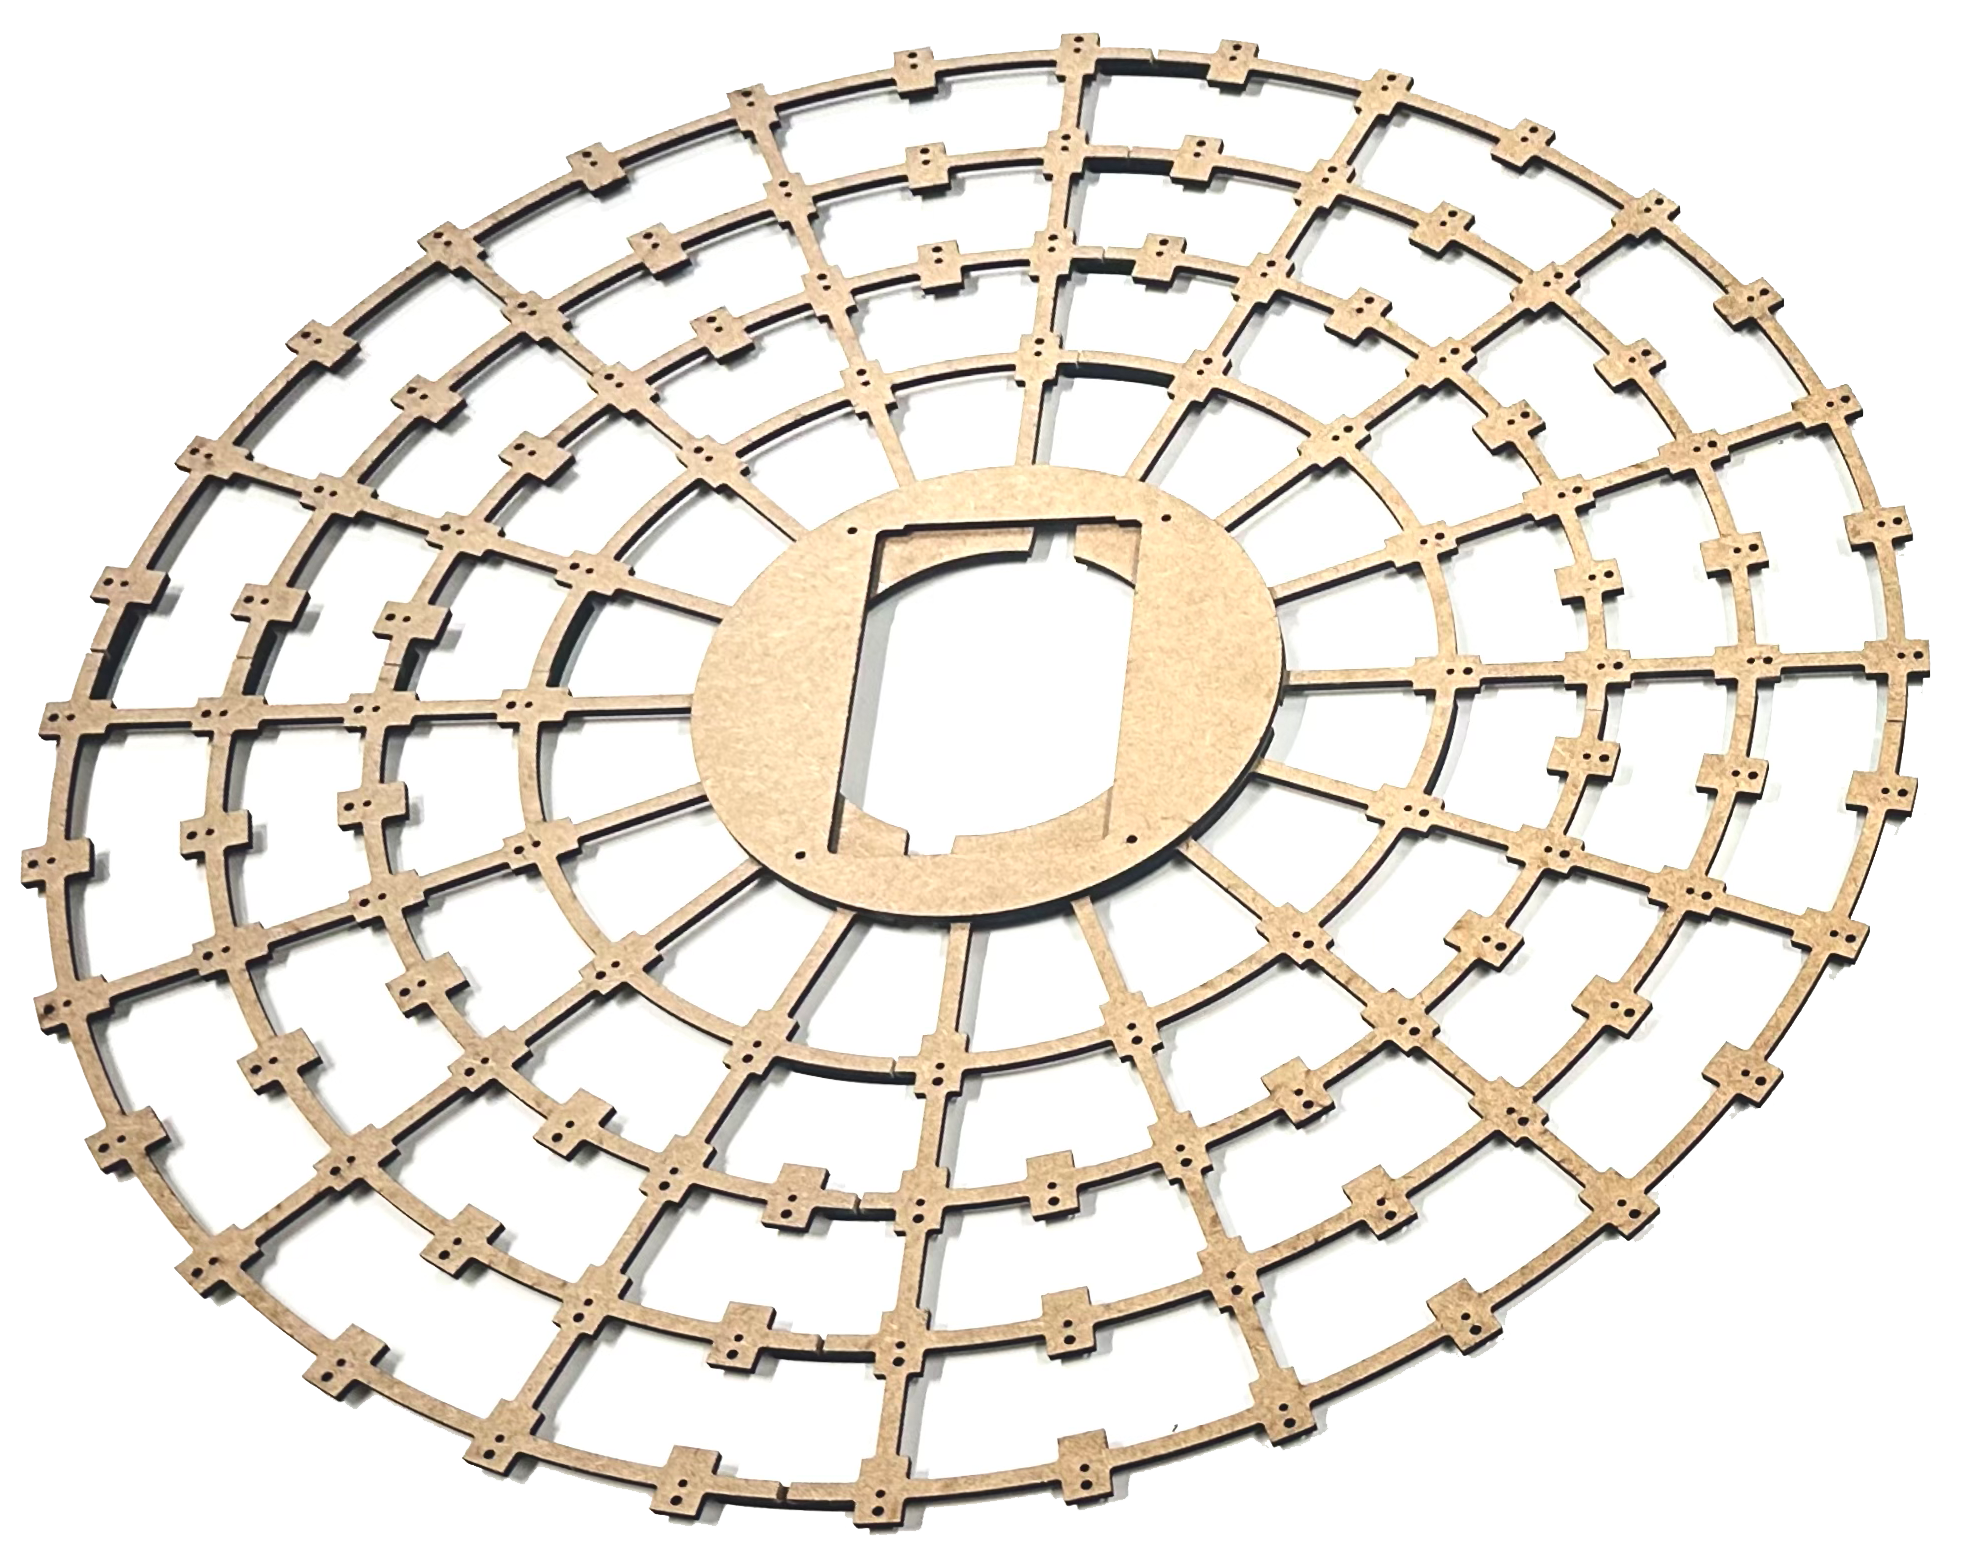
\includegraphics[width=0.95\textwidth]{images/5_array_evaluation/wooden_circular_array.png}
		\caption{Wooden Circular Array}
		\label{fig:wooden_circular_array}
	\end{minipage}
	\begin{minipage}{0.49\textwidth}
		\centering
		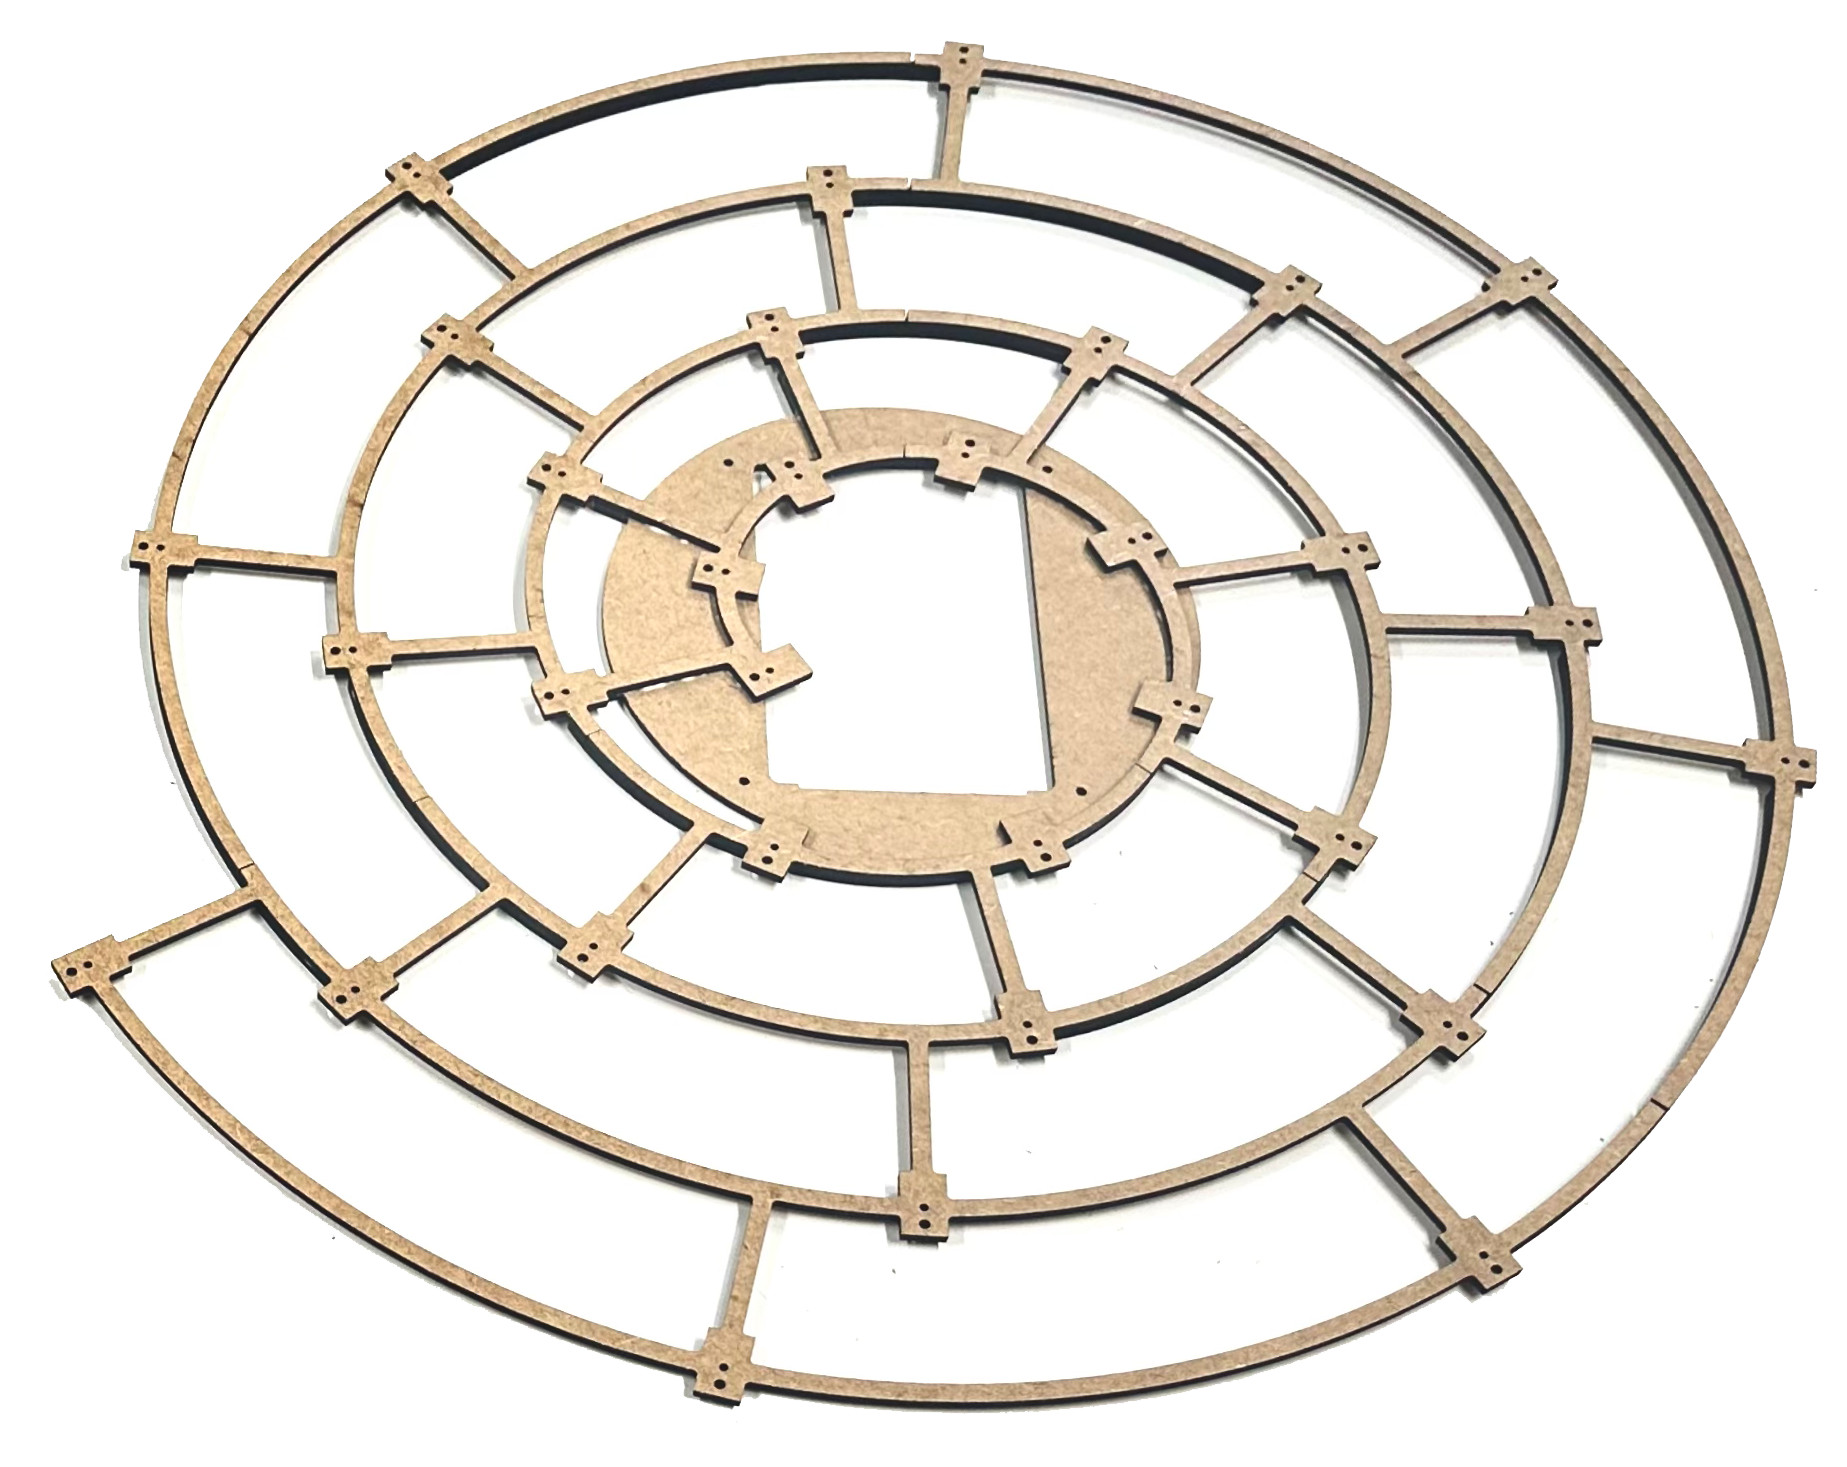
\includegraphics[width=0.95\textwidth]{images/5_array_evaluation/wooden_archimedean_spiral_array.png}
		\caption{Wooden Archimedean Spiral Array}
		\label{fig:wooden_archimedean_spiral_array}
	\end{minipage}
\end{figure}


\newpage
\section{Measurements \& Findings} \label{sec:array_prototype_measurements}
Blabla

\todo[inline]{Describe why we used fluffy stuff on the microphones (because we had problems first with wind). Mention the wind protection fur made by RØDE called DeadWombat.}


\begin{figure}[h!]
	\centering
	\begin{minipage}{0.49\textwidth}
		\centering
		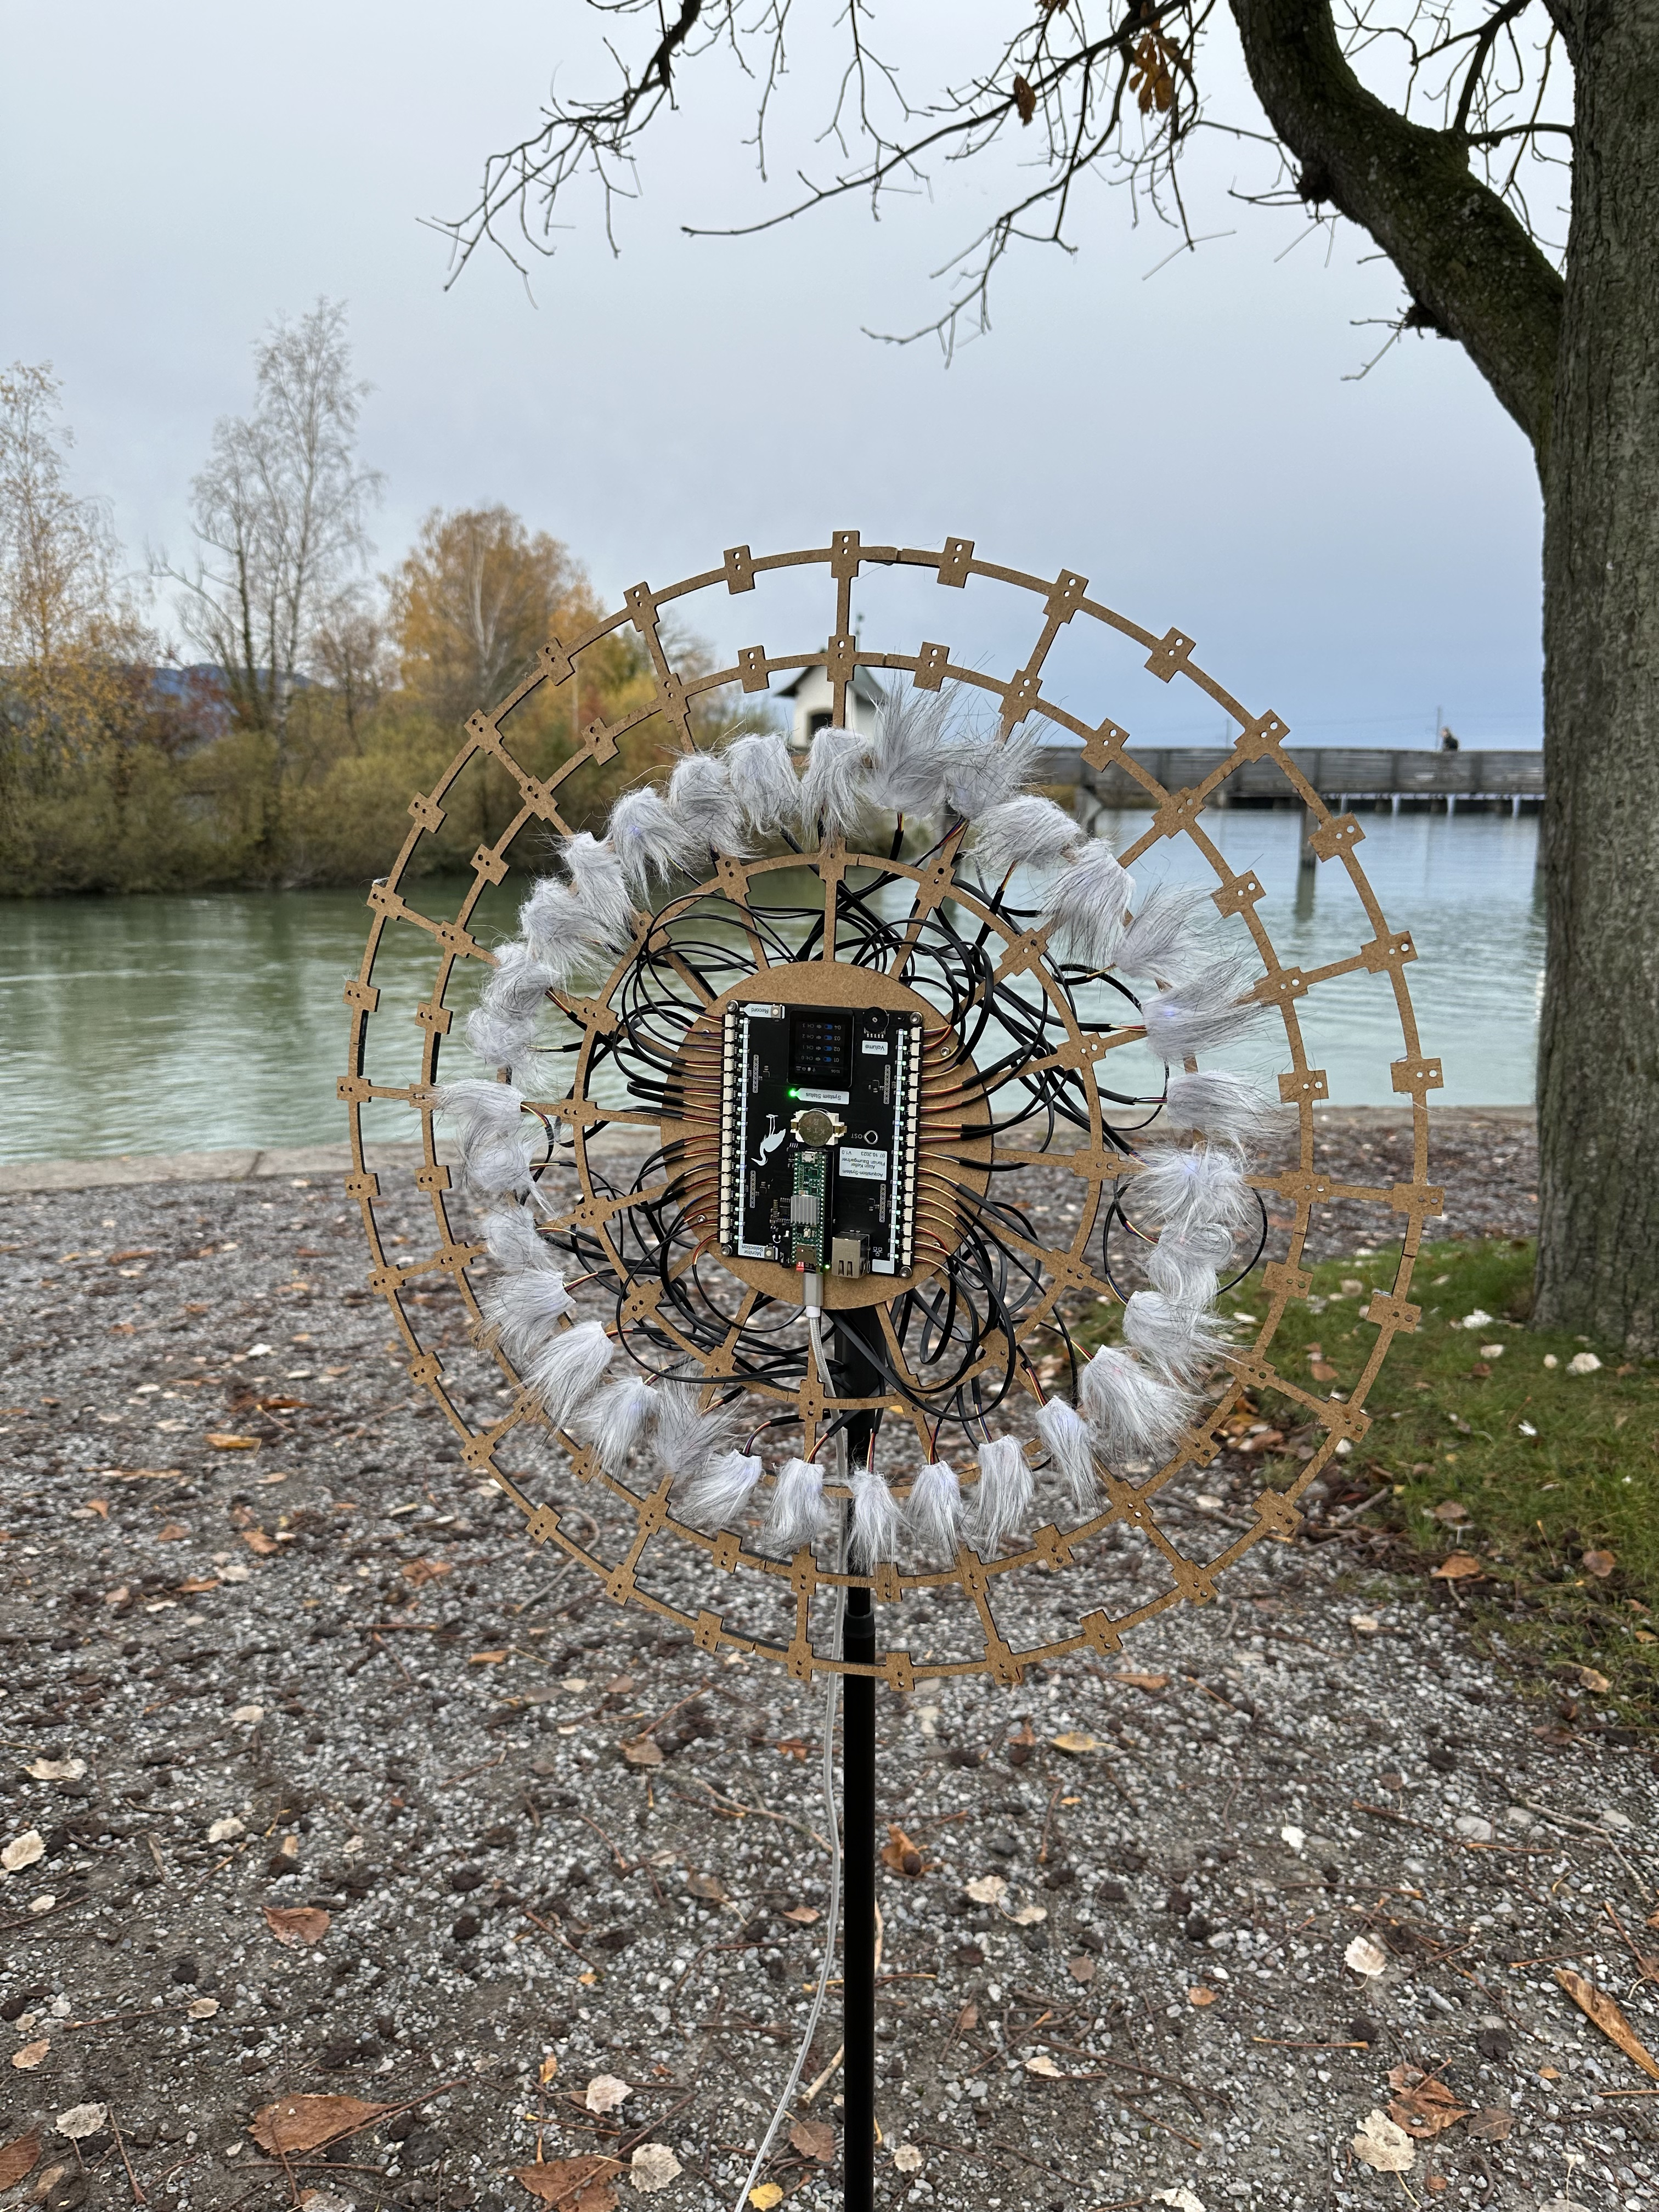
\includegraphics[width=0.95\textwidth]{images/5_array_evaluation/array_test_1.jpg}
		\caption{Multi-Circular Array (inner circle)}
		\label{fig:array_test_1}
	\end{minipage}
	\begin{minipage}{0.49\textwidth}
		\centering
		\includegraphics[width=0.95\textwidth]{images/5_array_evaluation/array_test_2.jpg}
		\caption{Multi-Circular Array (interleaved  pattern)}
		\label{fig:array_test_2}
	\end{minipage}
\end{figure}

\todo[inline]{Conclusion of array geometry → tree-dimensional array may provide better results. (This will be referenced in chapter of final design)}



\newpage
\section{Final Array Geometry} \label{sec:final_array_geometry}
Blabla

\begin{figure}[h]
	\centering
	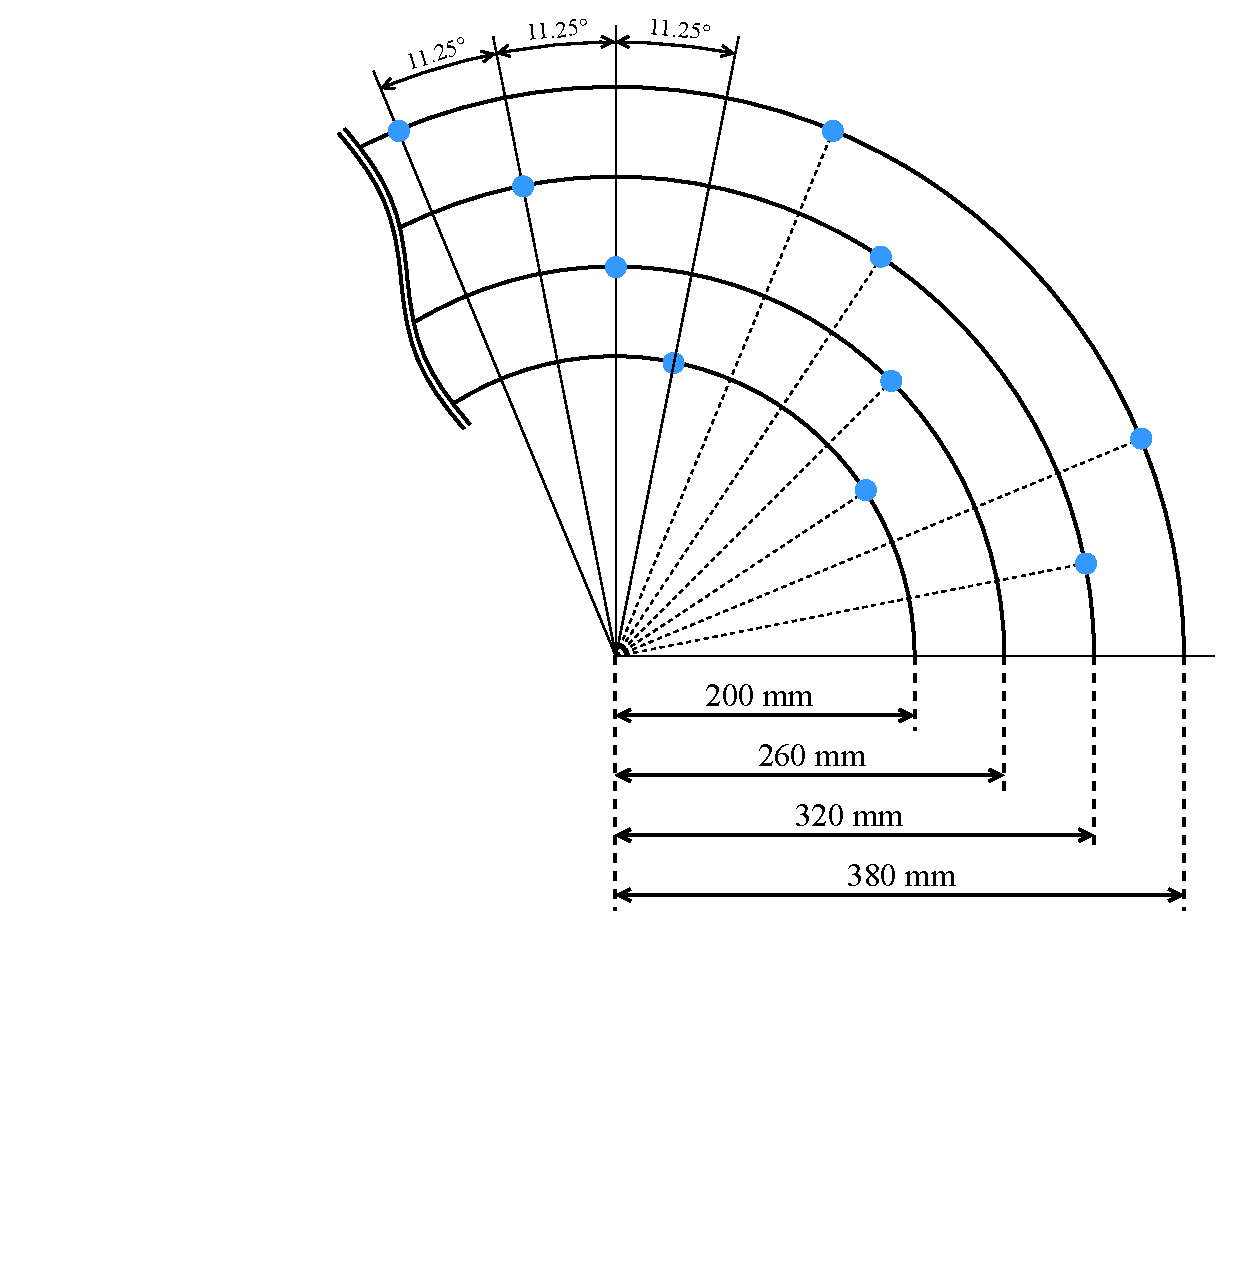
\includegraphics[width=0.75\textwidth, trim={5.5cm 6.0cm 0 0}]{images/5_array_evaluation/final_array_concept_design.pdf}
	\caption{Final Array Concept Design}
	\label{fig:final_array_concept_design}
\end{figure}

\chapter{Final Design}
\section{Overview}
This section covers the complete development process including the hardware, gateware, software and mechanical design of the project. It is important to note that the following documentation concentrates only on the final version of the device. Earlier hardware prototypes are not covered due to the lack of relevance.

\subsection{Key Requirements}
The main focus of the development is to design a professional looking, easy to use and eye-catching device for demonstration purposes. The project name \textit{Audio-Beamformer} has been chosen as it is easy to remember and has potential to be seen as a trademark.

The following key requirements have been set:
\begin{itemize}
	\item Single power adapter or power cable (e.g. no need of labor power supplies)
	\item Easy to install (e.g. montage on a camera tripod)
	\item Intuitive to operate via state-of-the-art graphical user interface
	\item Multiple audio streaming sources such as Bluetooth and USB input devices
	\item Great scalability and flexibility of the hardware and software design
\end{itemize}

\subsection{Key Decisions}
In the conceptional phase of the development, several key decisions had to be made. This contains mainly the signal flow and the division between the processing part on the Raspberry Pi and the \acrshort{fpga}. Further, the question had to be evaluated, if a built-in power supply or an external power adapter is preferred. And most importantly, which type of ultrasonic transducer should be used in the design.
In addition, the overall dimension and scale of the final product had to be discussed.
In general, most of these decisions were made according to results of simulations, physical measurements and after extensive discussions.
In the following sections, each part of the project is explained in detail.

\newpage
\section{Mechanical Design}
Blabla




\newpage
\section{Hardware Design}
Blabla

\begin{figure}
	\centering
	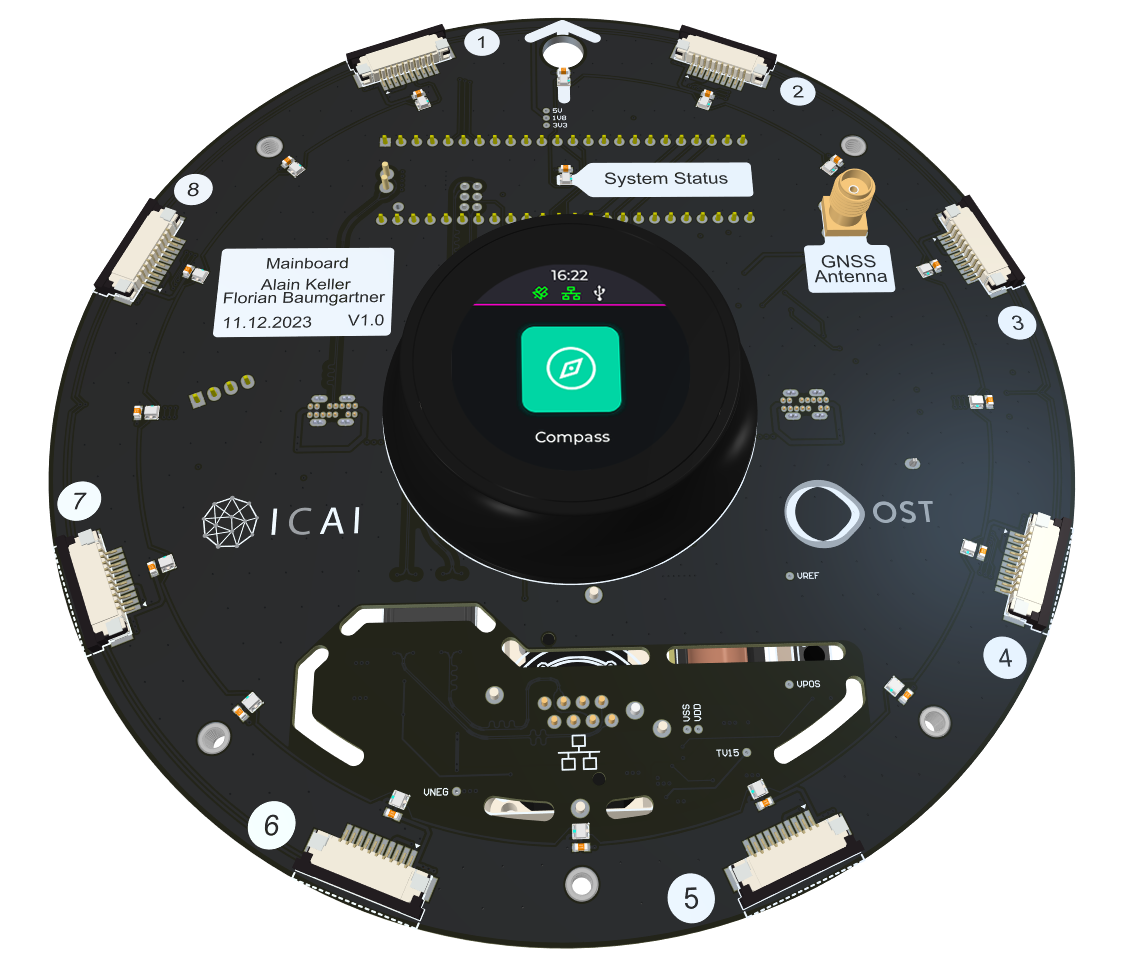
\includegraphics[width=1.0\textwidth]{images/6_design_final/Mainboard_Front_Display.png}
	\caption{Front view of the mainboard}
	\label{fig:mainboard_front}
\end{figure}




\subsection{Block Diagram}

\subsection{Power Supply}
The device can be powered by multiple sources. Primary the device is powered by the ethernet interface, which provides a \acrfull{poe} connection.
This is the preferred method, as it is the most convenient way to use the microphone array in the field.
In addition, there are two USB-C ports (\acrshort{mcu} and \acrshort{gnss}) that can be used to supply power when no PoE connection is available (e.g. in a laboratory environment for programming and debugging).
Each supply method can be used in conjunction with each other. However, the source must be able to provide at least 12.5\,W of power (5\,V, 2.5\,A).
In figure \ref{fig:power_supply_overview} an overview of the power supply is shown.
Note that the Teensy 4.1 has an internal 3.3\,V regulator, which is powered by the systems internal 5\,V supply.
The 1.8\,V rail is generated by a dedicated linear voltage regulator and is mainly used for the \acrshort{pdm} to \acrshort{tdm} converters (ADAU7118).

\begin{figure}
	\centering
	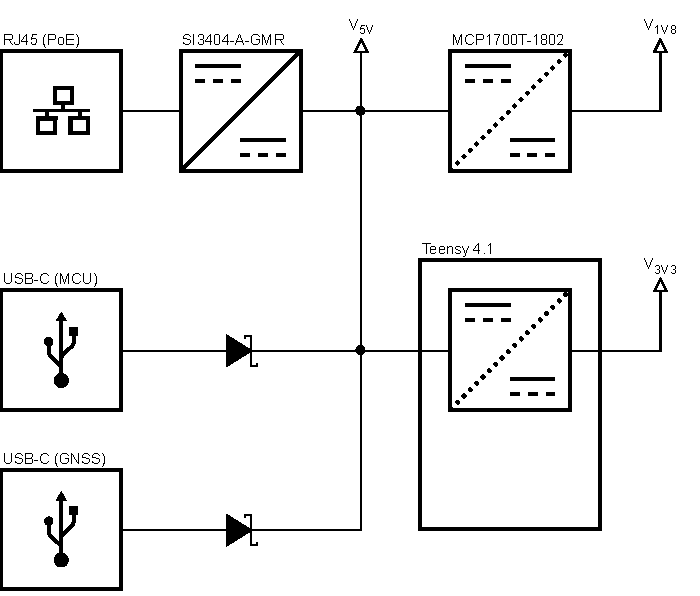
\includegraphics[width=0.65\textwidth]{images/6_design_final/final_design_power_supply.pdf}
	\caption{Power Supply Overview}
	\label{fig:power_supply_overview}
\end{figure}

\subsubsection{Power over Ethernet (PoE)}


\subsection{Microcontroller Unit (MCU)}

%  TODO: Write about external PSRAM

\subsection{Audio Input}

\subsubsection{GNSS}

\subsection{Human Machine Interface (HMI)}

%  TODO: Wite about LEDs and Buzzer

\subsubsection{LCD Display}

\subsubsection{RGB LEDs}

\subsection{Sensors}

\subsubsection{Magnetometer \& Accelerometer Sensor}

\subsubsection{Ambient Pressure \& Temperature Sensor}

\subsubsection{Angle Sensor}

\subsection{Printed Circuit Board (PCB)}

\subsubsection{Mainboard}

\subsubsection{Microphone Arms}

\subsubsection{Angle Sensor}

\subsection{Manufacturing}
The PCBs were manufactured and assembled by JLCPCB.
Only a few additional components were soldered by hand, such as the PDM to TDP converters (ADAU7118), the EtherCon connector and the GNSS module (NEO-M8P-2).
It turned out that multiple microphone arm PCBs were faulty (damaged microphones).
This was most likely caused by the soldering process, as the MEMS microphones are very sensitive to heat.

\newpage
\section{Firmware Design}
Blabla

\subsection{Overview}
The firmware is written in C++ and is based on the Arduino framework that has been addopted to the Teensy microcontroller environment.
As an IDE, the VS Code extension PlatfromIO was used, as it provides powerful development tools and a great integration of the Arduino framework.

The firmware is divided into modules running in individual threads, facilitated by TeensyThreads on the Teensy 4.1 microcontroller.
This lightweight multitasking library allows for concurrent execution of multiple threads, optimizing system performance and resource utilization.
TeensyThreads' minimal memory footprint and efficient CPU usage are critical in embedded systems where resources are constrained.


\begin{table}[h]
	\centering
	\begin{tabular}{|l|l|}
		\hline
		Thread                     & Purpose                      \\ \hline
		\texttt{Console Interface} & Handles USB virtual COM-Port \\ \hline
		\texttt{Console Streaming} & Handles queuing of messages  \\ \hline
		\texttt{Utils}             & Updates operation time       \\ \hline
		\texttt{AudioUtils}        & Audio Processing             \\ \hline
		\texttt{GNSS}              & GNSS Data Handling           \\ \hline
		\texttt{HMI}               & LED Control \& RTC           \\ \hline
		\texttt{Buzzer}            & Buzzer Control               \\ \hline
		\texttt{Application}       & Main Application Logic       \\ \hline
		\texttt{Main}              & Main Thread (Background)     \\ \hline
	\end{tabular}
	\caption{Overview of all threads and their purpose}
	\label{tab:threads}
\end{table}


\subsection{Audio Streaming}
The audio streaming module handles the buffering and transmission of the 32 audio channels.
It is based on a TCP server that provides a socket connection on port 6666.
The audio data is transmitted in a lossless 16-bit signed integer format, with a sample rate of 44.1 kHz.

The TCP connection asures a reliable data transmission, which is essential for the audio data.
To provide a low latency audio stream, the audio data is buffered in a circular buffer of 12 MB size.
This allows for a maximum delay of ca. 4.4\,s.

For a continuous audio stream, a tranmission rate of
\begin{equation}
	\frac{32\,\text{channels} \cdot 16\,\text{bit} \cdot 44100\,\text{Hz}}{10^6\,\text{bit/s}} = 22.1184\,\text{Mbit/s}
\end{equation}
is required.
The theoretical maximum transmission rate of 100Base-T Ethernet is 100\,Mbit/s.
However, the maximum transmission rate of the Teensy 4.1 is around 60\,Mbit/s, which is still sufficient for the audio stream.

Due to the maximal TCP packet size of 1460 bytes, the audio data is split into concatenated packets.
A frame consists of 128 interleafed samples (32 channels) and is transmitted in 8 packets.
Each frame starts with a 20-byte header.

\begin{table}[h]
	\centering
	\begin{tabular}{|l|l|l|l|}
		\hline
		\textbf{Byte Offset} & \textbf{Data Format}    & \textbf{Description} & \textbf{Example Value} \\ \hline
		0-7                  & String                  & Magic Sequence       & \codeword{HERON666}    \\ \hline
		8-11                 & Integer (Little Endian) & Packet Index         & 12345                  \\ \hline
		12-19                & Integer (Little Endian) & Timestamp (ns)       & 1616929134054668023    \\ \hline
	\end{tabular}
	\caption{Description of the 20-byte Packet Header}
	\label{tab:packet_header}
\end{table}

% TODO: Add frame example diagram
\begin{figure}[h]
	\centering
	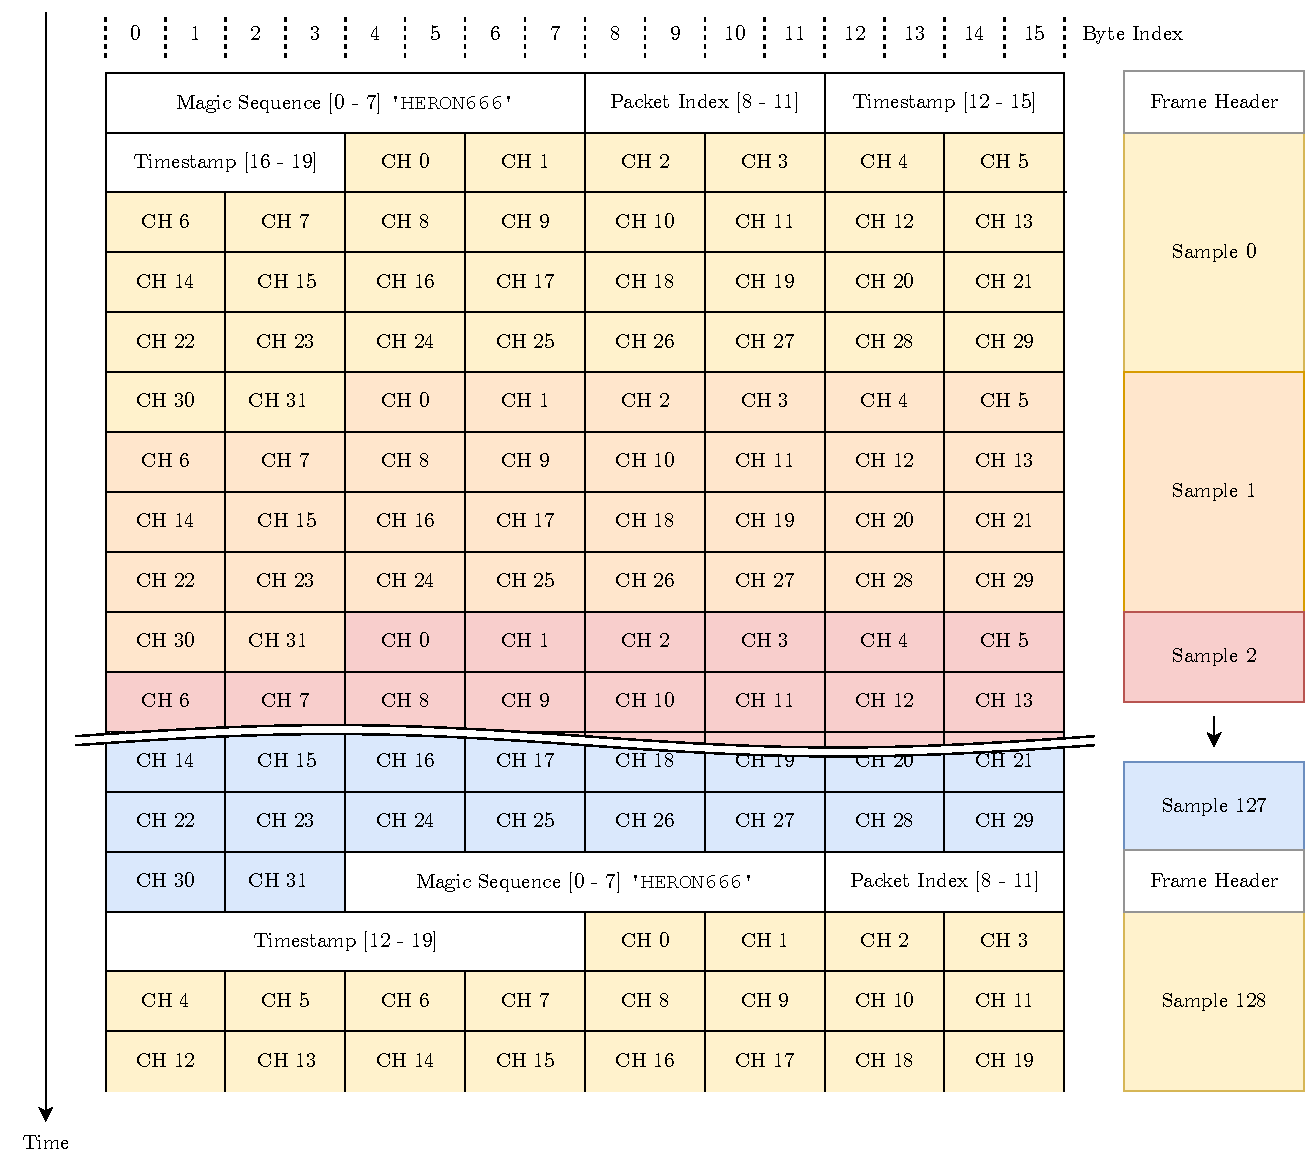
\includegraphics[width=1.0\textwidth]{images/6_design_final/Audio_Stream_Frame.pdf}
	\caption{Example of a Frame with 128 Samples (32 Channels)}
	\label{fig:frame_example}
\end{figure}

\subsubsection{Remote Configuration}
The

\begin{table}[h]
	\tiny
	\centering
	\begin{tabular}{|l|l|l|l|l|}
		\hline
		\textbf{Data Field}         & \textbf{Description}          & \textbf{Data Type} & \textbf{Unit} & \textbf{Example Value} \\ \hline
		device\_firmware\_version   & Firmware Version              & String             & -             & "V0.1"                 \\ \hline
		device\_firmware\_build     & Firmware Build Date           & String             & -             & "240110"               \\ \hline
		device\_cpu\_frequency      & CPU Frequency                 & Integer            & Hz            & 912000000              \\ \hline
		device\_cpu\_temperature    & Current CPU Temperature       & Float              & °C            & 36.5                   \\ \hline
		device\_operating\_time     & Device Operating Time         & Integer            & s             & 15615                  \\ \hline
		device\_system\_warning     & Current System Warning Status & Boolean            & -             & false                  \\ \hline
		ethernet\_mac               & MAC Address                   & String             & -             & "DE:AD:BE:EF:FE:ED"    \\ \hline
		ethernet\_ip                & Current IP Address            & String             & -             & "192.168.1.10"         \\ \hline
		streaming\_state            & Current Streaming State       & Boolean            & -             & true                   \\ \hline
		streaming\_speed            & Current Streaming Speed       & Float              & Mbit/s        & 22.21                  \\ \hline
		streaming\_buffer           & Streaming Buffer Fill Level   & Float              & \%            & 15.1                   \\ \hline
		sensor\_heading             & Device Heading                & Float              & °             & 270.0                  \\ \hline
		sensor\_pitch               & Device Pitch                  & Float              & °             & 5.2                    \\ \hline
		sensor\_roll                & Device Roll                   & Float              & °             & 2.4                    \\ \hline
		sensor\_temperature         & Ambient Temperature           & Float              & °C            & 22.3                   \\ \hline
		sensor\_pressure            & Ambient Pressure              & Float              & hPa           & 1013.2                 \\ \hline
		sensor\_altitude            & Device Altitude               & Float              & m (MSL)       & 434.5                  \\ \hline
		sensor\_angle               & Arm Angle                     & Float              & °             & 45.7                   \\ \hline
		sensor\_magnet\_detected    & Magnet Detection Status       & Boolean            & -             & true                   \\ \hline
		sensor\_magnet\_too\_weak   & Magnet Too Weak Status        & Boolean            & -             & false                  \\ \hline
		sensor\_magnet\_too\_strong & Magnet Too Strong Status      & Boolean            & -             & false                  \\ \hline
		gnss\_latitude              & GNSS Latitude                 & Float              & °             & 40.7128                \\ \hline
		gnss\_longitude             & GNSS Longitude                & Float              & °             & -74.0060               \\ \hline
		gnss\_altitude              & GNSS Altitude                 & Float              & m (MSL)       & 344.8                  \\ \hline
		gnss\_magnetic\_declination & GNSS Magnetic Declination     & Float              & °             & -5.0                   \\ \hline
		gnss\_satelite\_count       & GNSS Satellite Count          & Integer            & -             & 8                      \\ \hline
		gnss\_fix                   & GNSS Fix Status               & Boolean            & -             & true                   \\ \hline
		gnss\_fix\_type             & GNSS Fix Type                 & Integer            & -             & 3                      \\ \hline
		gnss\_time\_valid           & GNSS Time Validity            & Integer            & UNIX (UTC+0)  & 1704921651             \\ \hline
	\end{tabular}
	\caption{Device Data JSON File Fields, Descriptions, Data Types, Units, and Example Values}
	\label{table:device_data_types}
\end{table}


For remote configuration, the client (e.g. a PC) sends a JSON file containing the desired command and its parameters to the device.

\begin{table}[h]
	\tiny
	\centering
	\begin{tabular}{|l|l|l|l|l|}
		\hline
		\textbf{Data Field}    & \textbf{Description}                       & \textbf{Data Type} & \textbf{Unit} & \textbf{Example Value} \\ \hline
		clear\_warning         & Clears the warning status                  & Boolean            & -             & true / false           \\ \hline
		gnss\_coefficient\_xxx & GNSS RTK Coefficient XXX (Not implemented) & Float              & -             & -                      \\ \hline
	\end{tabular}
	\caption{Overview of Received Commands in JSON File}
	\label{tab:received_commands}
\end{table}

\subsection{Sensor Calibration}


\clearpage
\subsection{Graphical User Interface (GUI)}
The GUI provides a user-friendly interface for configuring the device and monitoring its status.
It is based on the LVGL framework.



\clearpage
\subsection{GUI Pages}
In the following sections, the different GUI pages are explained in detail.
Navigating between the pages is done by clicking on the corresponding icon in the home menu.
To return to the home menu, the sub-page header bar with the arrow symbol can be pressed.
Figure \ref{fig:gui_pages_overview} shows an overview of all GUI pages and how navigation between them is done.
\begin{figure}[h]
	\centering
	\vspace{-0.5cm}
	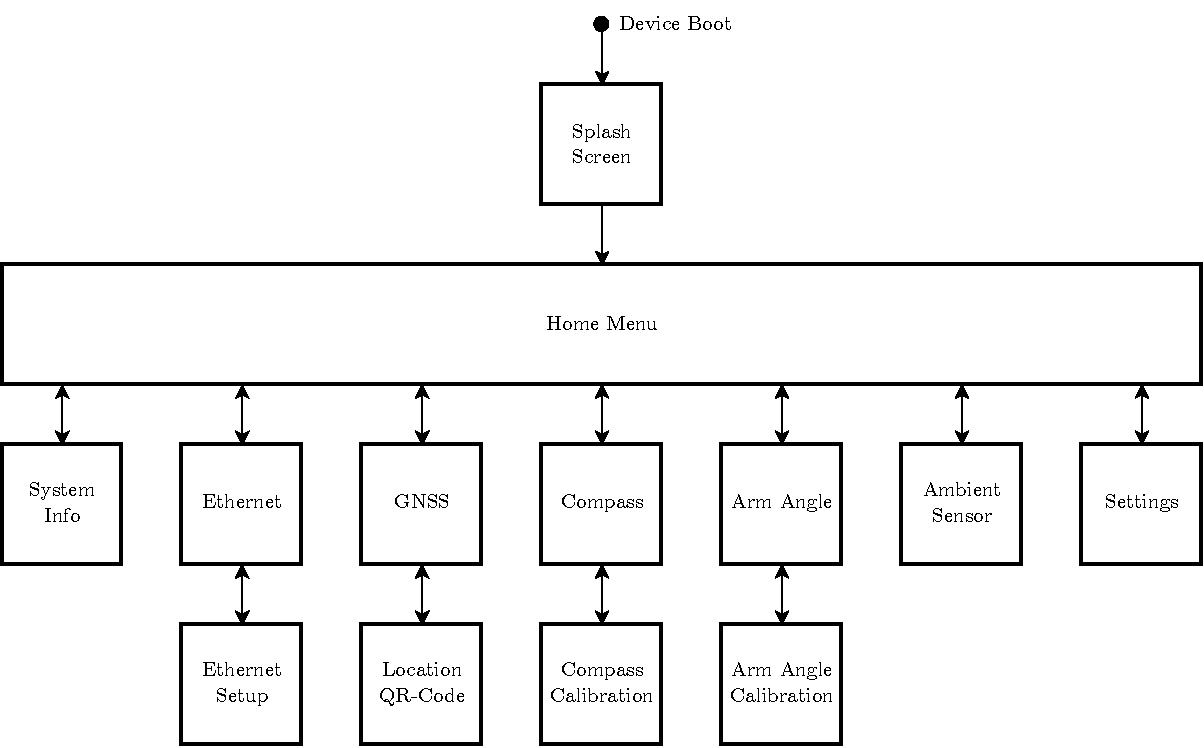
\includegraphics[width=0.85\textwidth]{images/6_design_final/final_design_gui_pages.pdf}
	\caption{GUI Pages Overview}
	\label{fig:gui_pages_overview}
\end{figure}
\vspace{-0.3cm}

\begin{minipage}{\linewidth}
	\begin{wrapfigure}{l}{4.5cm}
		\vspace{-0.6cm}
		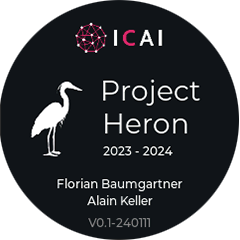
\includegraphics[width=4cm]{images/6_design_final/gui/00_splash_screen.png}
		\centering
		\caption{Splash Screen}
		\label{fig:final_design_gui_splash_screen}
	\end{wrapfigure}
	\subsubsection{Splash Screen}
	When the system is powered on, the splash screen is displayed for 5 seconds.
	On the bottom of the screen, the current firmware version and build date is displayed.
	After the system has booted, the home menu is displayed.
\end{minipage}
\vspace{2.2cm}		% One line corresponds to ca. 0.4cm

\begin{minipage}{\linewidth}
	\begin{wrapfigure}{l}{4.5cm}
		\vspace{-0.6cm}
		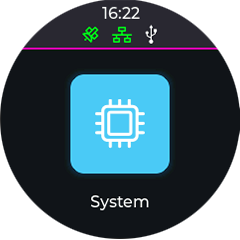
\includegraphics[width=4cm]{images/6_design_final/gui/01_main_menu.png}
		\centering
		\caption{Home Menu}
		\label{fig:final_design_gui_home_menu}
	\end{wrapfigure}
	\subsubsection{Home Menu}
	The home menu presents an intuitive way of navigating through the different submenus.
	On the top of the screen, the current time is displayed.
	A dedicated icon for the \acrshort{gnss}, ethernet and \acrshort{usb} interface is shown.
	Per default, the icons are grayed out.
	When the \acrshort{gnss} location is valid (fix), the icon turns green.
	When the device is connected to the network but is not yet streaming, the icon is filled white.
	As soon as the audio stream is active, the icon turns green.
	The \acrshort{usb} icon is filled white when a device is connected to the \acrshort{usb} port.
	As soon as the virtual COM port is opened, the icon turns green.
\end{minipage}
\pagebreak

\begin{minipage}{\linewidth}
	\begin{wrapfigure}{l}{4.5cm}
		\vspace{-0.6cm}
		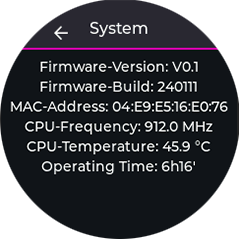
\includegraphics[width=4cm]{images/6_design_final/gui/03_system_info.png}
		\centering
		\caption{System Information}
		\label{fig:final_design_gui_system_info}
	\end{wrapfigure}
	\subsubsection{System Information}
	The system information page displays important device information such as the firmware version,
	firmware build date, etherent \acrshort{mac} address, \acrshort{cpu} frequency and temperature, as well as the operating time.
\end{minipage}
\vspace{1.3cm}

\begin{minipage}{\linewidth}
	\begin{wrapfigure}{l}{4.5cm}
		\vspace{-0.6cm}
		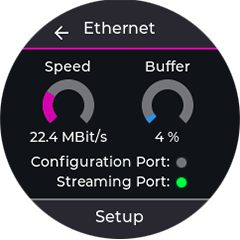
\includegraphics[width=4cm]{images/6_design_final/gui/04_ethernet.png}
		\centering
		\caption{Ethernet}
		\label{fig:final_design_gui_ethernet}
	\end{wrapfigure}
	\subsubsection{Ethernet}
	The ethernet page displays the current connection state of the streaming and configuration port.
	While a connection is established to either of the ports, the corresponding gray circle is filled green.
	Two gauge bars display the current streaming speed and the fill level of the streaming buffer.
	In normal operation, the indicated streaming speed should be around 22\,Mbit/s and the buffer fill level near 0\,\%.
\end{minipage}
\vspace{0.0cm}

\begin{minipage}{\linewidth}
	\begin{wrapfigure}{l}{4.5cm}
		\vspace{-0.6cm}
		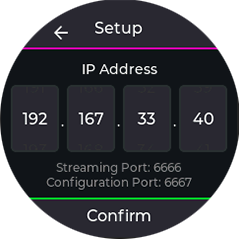
\includegraphics[width=4cm]{images/6_design_final/gui/05_ethernet_config.png}
		\centering
		\caption{Ethernet Setup}
		\label{fig:final_design_gui_ethernet_setup}
	\end{wrapfigure}
	\subsubsection{Ethernet Setup}
	The ethernet setup page allows for configuring the \acrshort{ip} address  of the device.
	Below the \acrshort{ip} address, the hard-coded streaming port (6666) and configuration port (6667) is displayed.
	When the \acrshort{ip} address is changed, the user can either confirm the change or discard it by returning to the previous page.
	When a new \acrshort{ip} address is confirmed, the device will instantly change its \acrshort{ip} address and restart the servers.
\end{minipage}
\vspace{0.0cm}

\begin{minipage}{\linewidth}
	\begin{wrapfigure}{l}{4.5cm}
		\vspace{-0.6cm}
		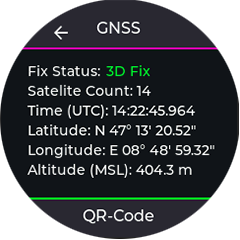
\includegraphics[width=4cm]{images/6_design_final/gui/06_gnss.png}
		\centering
		\caption{GNSS}
		\label{fig:final_design_gui_gnss}
	\end{wrapfigure}
	\subsubsection{GNSS}
	The \acrshort{gnss} page displays the current status of the \acrshort{gnss} module.
	When the Fix Status is valid (2D-Fix or 3D-Fix), the latitude, longitude and altitude is displayed.
	In addition, the QR-Code button gets enabled, which allows for displaying the current location in a QR-Code.
	The coordinates are displayed in degrees, minutes and seconds.
	The altitude is displayed in meters above sea level (MSL).
	When the time is fully resolved, it is displayed in the UTC+0 format.
	While the Fix Status is invalid, all fields are grayed out.
\end{minipage}
\vspace{0.0cm}

\begin{minipage}{\linewidth}
	\begin{wrapfigure}{l}{4.5cm}
		\vspace{-0.6cm}
		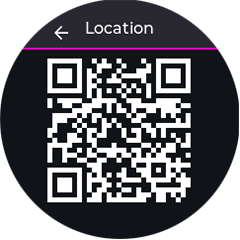
\includegraphics[width=4cm]{images/6_design_final/gui/07_gnss_location.png}
		\centering
		\caption{Location QR-Code}
		\label{fig:final_design_gui_gnss}
	\end{wrapfigure}
	\subsubsection{GNSS Location QR-Code}
	The \acrshort{gnss} location \acrshort{qr}-Code page displays a \acrshort{qr}-Code containing a google maps link to the current location.
	When the \acrshort{qr}-Code is scanned with a smartphone, the web broweser will immediately redirect the user to the google maps app.
	The \acrshort{url} is formated as follows: \smallskip \newline
	\codeword{google.com/maps/place/<latitude>,<longitude>} \smallskip \newline
	For example, the \acrshort{url} directs to: \smallskip \newline
	\url{google.com/maps/place/47.222400,8.816460}
\end{minipage}
\vspace{-0.2cm}

\begin{minipage}{\linewidth}
	\begin{wrapfigure}{l}{4.5cm}
		\vspace{-0.6cm}
		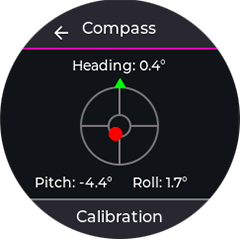
\includegraphics[width=4cm]{images/6_design_final/gui/08_compass.png}
		\centering
		\caption{Compass}
		\label{fig:final_design_gui_compass}
	\end{wrapfigure}
	\subsubsection{Compass}
	The compass page displays the current heading and leveling of the device.
	The heading is indicated by a purple arrow, pointing towards geographic north.
	When the needle points exactly towards the top of the screen it turns green, meaning the device is facing north.
	The circular graphic in the centre of the screen shows the current leveling of the device.
	When the device is perfectly leveled, the circle turns green.
	When the device is tilted, the circle turns red and the tilt angle is displayed in degrees (pitch and roll).
	To calibrate the built-in magnetometer, the user can press the calibrate button.
\end{minipage}
\vspace{-0.2cm}

\begin{minipage}{\linewidth}
	\begin{wrapfigure}{l}{4.5cm}
		\vspace{-0.6cm}
		\includegraphics[width=4cm]{images/6_design_final/gui/09_compass_calibration.png}
		\centering
		\caption{Compass Calib.}
		\label{fig:final_design_gui_compass_calibration}
	\end{wrapfigure}
	\subsubsection{Compass Calibration}
	The compass calibration page displays the current status of the magnetometer calibration.
	By entering this page, the calibration process is starts immediately.
	To calibrate the magnetometer, the device has to be rotated around all three axes.
	This process takes around 30 seconds.
	As soon as the spere coverage indicator reaches 100\,\%, the calibration is finished, a success message is displayed and the buzzer plays a short melody.
	The calibration process can be aborted at any time by returning to the previous page (the calibration progress is not saved).
\end{minipage}
\vspace{-0.2cm}

\begin{minipage}{\linewidth}
	\begin{wrapfigure}{l}{4.5cm}
		\vspace{-0.6cm}
		\includegraphics[width=4cm]{images/6_design_final/gui/10_angle_sensor.png}
		\centering
		\caption{Arm Angle}
		\label{fig:final_design_gui_arm_angle}
	\end{wrapfigure}
	\subsubsection{Arm Angle}
	The arm angle page displays the current angle of the microphone array arms in degree.
	When the arms are fully unfolded (horizontal) the angle is 0.0\,°.
	When the arms are fully folded towards the centre pole the angle is 90.0\,°.
	Below the angle indicator, the current status of the magnet detection is displayed.
	When the magnet is detected, the status indicator turns green.
	If the magnet is too weak or too strong, the corresponding status indicator turns yellow.
	Otherwise, the status indicators are grayed out.
\end{minipage}
\pagebreak

\begin{minipage}{\linewidth}
	\begin{wrapfigure}{l}{4.5cm}
		\vspace{-0.6cm}
		\includegraphics[width=4cm]{images/6_design_final/gui/11_angle_sensor_calibration.png}
		\centering
		\caption{Arm Angle Calib.}
		\label{fig:final_design_gui_arm_angle_calibration}
	\end{wrapfigure}
	\subsubsection{Arm Angle}
	The arm angle calibration page lets the user calibrate the angle sensor.
	To calibrate the angle sensor, the arms have to be fully unfolded (horizontal).
	Then the upper calibrate button \textit{Calibrate 0° (unfolded)} has to be pressed.
	Next, the arms have to be fully folded towards the centre pole.
	Then the lower calibrate button \textit{Calibrate 90° (folded)} has to be pressed.
	To confirm the calibration, the user has to press the \textit{Confirm} button.
\end{minipage}
\vspace{0.0cm}

\begin{minipage}{\linewidth}
	\begin{wrapfigure}{l}{4.5cm}
		\vspace{-0.6cm}
		\includegraphics[width=4cm]{images/6_design_final/gui/12_ambient_sensor.png}
		\centering
		\caption{Ambient Sensor}
		\label{fig:final_design_gui_ambient_sensor}
	\end{wrapfigure}
	\subsubsection{Ambient Sensor}
	The ambient sensor page displays the current ambient temperature in degree Celsius and the ambient pressure in hectopascal.
	A gauge bar visualizes both values.
	Based on the current ambient pressure, the altitude above sea level is calculated and displayed in meters.
	Note that the altitude is only an approximation and can be inaccurate.
	It is strongly influenced by the current weather conditions.
\end{minipage}
\vspace{0.5cm}

\begin{minipage}{\linewidth}
	\begin{wrapfigure}{l}{4.5cm}
		\vspace{-0.6cm}
		\includegraphics[width=4cm, trim={0 -1.0cm 0 0}]{images/6_design_final/gui/13_settings.png}
		\includegraphics[width=4cm]{images/6_design_final/gui/14_settings.png}
		\centering
		\caption{Settings}
		\label{fig:final_design_gui_settings}
	\end{wrapfigure}
	\subsubsection{Settings}
	The settings page allows the user to configure the device.
	First, the buzzer can be enabled or disabled.
	Second, the \acrshort{led}s can be permanently enabled or disabled.
	The mode selection provides a selection of different animations for the \acrshort{led}s.
	Currently, there are two animation types implemented:
	\begin{itemize}
		\setlength{\itemindent}{5mm}
		\setlength{\leftmargin}{10mm}
		\item \textbf{Audio:} The \acrshort{led}s are controlled by the audio level of the microphone array.
		\item \textbf{OST:} The \acrshort{led}s show a fluent animation in the \acrshort{ost} color scheme.
	\end{itemize}
	Below the mode settings, the \acrshort{led} brightness can be adjusted.
	All settings are saved in the internal flash memory of the device and are restored after a reboot.
\end{minipage}


\newpage
\section{Software Design}
Blabla





\chapter{Measurements}
\section{Overview}
This section covers the complete development process including the 
hardware, gateware, software and mechanical design of the project. 
It is important to note that the following documentation concentrates 
only on the final version of the device. 
Earlier hardware prototypes are not covered due to the lack of relevance.

The measurements were performed in an open filed with a 
DJI Mavic Pro drone.
\subsection{Stationary drone}
In the stationary drone test, the drone flew to different points,
where it then stayed still.
For the test five points in different directions were chosen.
Table \ref*{meas:tabP} shows these five points.
These points were measured using the GPS of the drone 
so their position are not known with great precision.
At each of the five points the array was tested with five 
different arm angles. 

\begin{table}[h]
    \centering
    \begin{tabular}{ |c"c|c|c| }    
        \hline
        * & \makecell{$\phi_s$} & 
        \makecell{$\theta_s$} & 
        \makecell{$r_s$}\\
        \thickhline
            $\bm{P_1}$ & 
            \makecell{$-120^\circ$} & 
            \makecell{$70^\circ$}& 
            \makecell{$31$m}\\ 
        \hline
            $\bm{P_2}$ & 
            \makecell{$-158^\circ$}& 
            \makecell{$50^\circ$}& 
            \makecell{$17$m}\\ 
        \hline
            $\bm{P_3}$ & 
            \makecell{$-158^\circ$}& 
            \makecell{$25^\circ$}& 
            \makecell{$32$m}\\ 
        \hline
            $\bm{P_4}$ & 
            \makecell{$-158^\circ$}&
            \makecell{$15^\circ$}& 
            \makecell{$52$m}\\
        \hline
            $\bm{P_5}$ & 
            \makecell{$0^\circ$}&
            \makecell{$0^\circ$}& 
            \makecell{$50$m}\\
        \hline
    \end{tabular}
    \caption{Postions of the test points.}
    \label{meas:tabP}
\end{table}

The measurements include the calculated \acrshort*{doa} and the two metrics introduced
in section \ref{sec:metrics}.
Tables \ref*{meas:tabPhi} and \ref*{meas:tabtheta} show the signed error
for the two angles $\phi$ and $\theta$.
The measurement of $\phi$ is relatively independent of the array arm angle.
However for positions with a high $\theta_s$ the error in $\theta$ increases
when the arm angle increases. 
Since this was not the case in the simulation, it is suspected that 
these errors come from physical effects of the sound waves in the array 
and the directionality of the used microphones.

\begin{table}[h]
    \centering
    \begin{tabular}{ |P{1.8cm}"l|l|l|l|l | }
        \hline
        Arm angle & \makecell{$\bm{P}_1$} & 
        \makecell{$\bm{P}_2$} & 
        \makecell{$\bm{P}_3$} & 
        \makecell{$\bm{P}_4$} & 
        \makecell{$\bm{P}_5$}\\
        \thickhline
            $0^\circ$ & 
            $-2^\circ$& 
            \makecell{$+5^\circ$}& 
            \makecell{$+2^\circ$}& 
            \makecell{$+3^\circ$}&
            \makecell{$0^\circ$}\\ 
        \hline
            $15^\circ$ & 
            \makecell{$-2^\circ$} & 
            \makecell{$-1^\circ$}& 
            \makecell{$+0^\circ$}& 
            \makecell{$+2^\circ$}&
            \makecell{$+0^\circ$}\\ 
        \hline
            $30^\circ$ & 
            \makecell{$-2^\circ$} & 
            \makecell{$+6^\circ$}& 
            \makecell{$+1^\circ$}& 
            \makecell{$+4^\circ$}&
            \makecell{$+0^\circ$}\\ 
        \hline
            $45^\circ$ & 
            \makecell{$-1^\circ$} & 
            \makecell{$+6^\circ$}& 
            \makecell{$+2^\circ$}& 
            \makecell{$+5^\circ$}&
            \makecell{$+0^\circ$}\\ 
        \hline
            $60^\circ$ &
            \makecell{$-2^\circ$} & 
            \makecell{$+6^\circ$}& 
            \makecell{$+4^\circ$}& 
            N/A&
            N/A\\
        \hline
    \end{tabular}
    \caption{Signed error in $\phi$.
    The errors for $\bm{P}_5$ are 0 due to its indefiniteness when $\theta = 0$.}
    \label{meas:tabPhi}
\end{table}

\begin{table}[h]
    \centering
    \begin{tabular}{ |P{1.8cm}"l|l|l|l|l | }
        \hline
        Arm angle & \makecell{$\bm{P}_1$} & 
        \makecell{$\bm{P}_2$} & 
        \makecell{$\bm{P}_3$} & 
        \makecell{$\bm{P}_4$} & 
        \makecell{$\bm{P}_5$}\\
        \thickhline
            $0^\circ$ & 
            \makecell{$+2^\circ$} & 
            \makecell{$+5^\circ$}& 
            \makecell{$+0^\circ$}& 
            \makecell{$+0^\circ$}&
            \makecell{$+1^\circ$}\\ 
        \hline
            $15^\circ$ & 
            \makecell{$+5^\circ$} & 
            \makecell{$+5^\circ$}& 
            \makecell{$+0^\circ$}& 
            \makecell{$+0^\circ$}&
            \makecell{$+1^\circ$}\\ 
        \hline
            $30^\circ$ & 
            \makecell{$+10^\circ$} & 
            \makecell{$+9^\circ$}& 
            \makecell{$+1^\circ$}& 
            \makecell{$+0^\circ$}&
            \makecell{$+1^\circ$}\\ 
        \hline
            $45^\circ$ & 
            \makecell{$+20^\circ$} & 
            \makecell{$+10^\circ$}& 
            \makecell{$+1^\circ$}& 
            \makecell{$+0^\circ$}&
            \makecell{$+1^\circ$}\\ 
        \hline
            $60^\circ$ &
            \makecell{$+20^\circ$} & 
            \makecell{$+11^\circ$}& 
            \makecell{$+2^\circ$}& 
            N/A&
            N/A\\
        \hline
    \end{tabular}
    \caption{Signed error in $\theta$.}
    \label{meas:tabtheta}
\end{table}

The mainlobe areas from the measurements are as expected from the simulations.
It is however observed that the mainlobe area at $\bm{P}_1, \bm{P}_3$ and $\bm{P}_4$
is better when the arm is angled. 
WIth the current measurements it can not be stated if this results from noise or
from other effects.

The PAP ratio is significantly lower than in the simulated cases.
Since the measurement was taken outdoors with background noise, 
this is no surprise.
Nonetheless the PAP ratio follows similar trends when $\theta_s$ or the arm angle is changed.
\begin{table}[h]
    \centering
    \begin{tabular}{ |P{1.8cm}"P{2cm}|P{2cm}|P{2cm}|P{2cm}|P{2cm} | }
        \hline
        Arm angle & \makecell{$\bm{P}_1$} & 
        \makecell{$\bm{P}_2$} & 
        \makecell{$\bm{P}_3$} & 
        \makecell{$\bm{P}_4$} & 
        \makecell{$\bm{P}_5$}\\
        \thickhline
            $0^\circ$ & 
            \makecell{$4.85\%$} & 
            \makecell{$4.37\%$}& 
            \makecell{$2.42\%$}& 
            \makecell{$2.90$\%}&
            \makecell{$1.45\%$}\\ 
        \hline
            $15^\circ$ & 
            \makecell{$4.24\%$} & 
            \makecell{$4.52\%$}& 
            \makecell{$2.01\%$}& 
            \makecell{$1.82\%$}&
            \makecell{$2.00\%$}\\ 
        \hline
            $30^\circ$ & 
            \makecell{$4.15\%$} & 
            \makecell{$6.71\%$}& 
            \makecell{$2.92\%$}& 
            \makecell{$2.30\%$}&
            \makecell{$1.82\%$}\\ 
        \hline
            $45^\circ$ & 
            \makecell{$4.10\%$} & 
            \makecell{$6.62\%$}& 
            \makecell{$4.62\%$}& 
            \makecell{$2.95\%$}&
            \makecell{$2.31\%$}\\ 
        \hline
            $60^\circ$ &
            \makecell{$4.26\%$} & 
            \makecell{$6.76\%$}& 
            \makecell{$5.16\%$}& 
            N/A&
            N/A\\
        \hline
    \end{tabular}
    \caption{Mainlobe area ratio at the testpoints.}
    \label{meas:tabarea}
\end{table}

\begin{table}[h]
    \centering
    \begin{tabular}{ |P{1.8cm}"P{2cm}|P{2cm}|P{2cm}|P{2cm}|P{2cm} | }
        \hline
        Arm angle & \makecell{$\bm{P}_1$} & 
        \makecell{$\bm{P}_2$} & 
        \makecell{$\bm{P}_3$} & 
        \makecell{$\bm{P}_4$} & 
        \makecell{$\bm{P}_5$}\\
        \thickhline
            $0^\circ$ & 
            \makecell{$7.17$} & 
            \makecell{$10.20$}& 
            \makecell{$12.23$}& 
            \makecell{$7.65$}&
            \makecell{$16.82$}\\ 
        \hline
            $15^\circ$ & 
            \makecell{$9.30$} & 
            \makecell{$9.95$}& 
            \makecell{$11.81$}& 
            \makecell{$13.94$}&
            \makecell{$14.51$}\\ 
        \hline
            $30^\circ$ & 
            \makecell{$9.45$} & 
            \makecell{$8.35$}& 
            \makecell{$10.61$}& 
            \makecell{$11.30$}&
            \makecell{$13.45$}\\ 
        \hline
            $45^\circ$ & 
            \makecell{$9.14$} & 
            \makecell{$7.98$}& 
            \makecell{$7.74$}& 
            \makecell{$8.26$}&
            \makecell{$11.56$}\\ 
        \hline
            $60^\circ$ &
            \makecell{$9.68$} & 
            \makecell{$8.34$}& 
            \makecell{$5.16$}& 
            N/A&
            N/A\\
        \hline
    \end{tabular}
    \caption{PAP ratio at the testpoints.}
    \label{meas:tabPap}
\end{table}

\subsection{Moving drone test}
Making a verifiable test for a flying drone was not possible due to 
a lack of time.
To test the localization and tracking of a flying drone qualitative
tests were performed.
For the test the drone flew along paths in the test environment.
Ideally the track created by the drone is parallel to these paths.
To check the $\theta$ angle, the same track was flew in different height.
A comparison of two such flights are shown in Figure \ref*{meas:fig:west east}.
In Figure \ref*{meas:fig:west east high}, it is apparent that when the drone ascended by 10 meters, 
the measured $\theta$ was lower than in Figure \ref*{meas:fig:west east low}, as anticipated.

\begin{figure}[h]
	\centering
	\begin{subfigure}[t]{0.45\textwidth}
		\centering
		\includegraphics[width=\textwidth]{images/7_measurements/we_low.png}
		\caption{Drone flies in $40$m elevation}
		\label{meas:fig:west east low}
	\end{subfigure}
	\hfill
	\begin{subfigure}[t]{0.45\textwidth}
		\centering
		\includegraphics[width=\textwidth]{images/7_measurements/we_high.png}
		\caption{Drone flies in $50$m elevation}
		\label{meas:fig:west east high}
	\end{subfigure}
	\caption{Drone flying along the road from west to east in two different
    elevations.
    The distance between the red center point and the track is linearly 
    dependent on $\theta$ whereas the angle between east and the track represents $\phi$.
    The thicker point right of the tracks shows the current tracker positions.}
	\label{meas:fig:west east}
\end{figure}

\chapter{Conclusion}
In conclusion, this thesis has delved into the task of 
localizing and tracking a drone utilizing a microphone array. 
Through a comprehensive evaluation of both software and hardware aspects,
new insights into the field had been gained, and
a custom built system has been developed.
With qualitative and quantitative measurements it has been shown, 
that the proposed system is able to localize and track 
drones in the open field.

\section{Continuing Work}

\bigskip
\begin{itemize}
		\item Build additional two arrays to allow exact localization
		\item Integrating a camera to visually show the drone's position
		\item Improve computation time of the beamforming
		\item More elaborate testing
		\item Evaluating different trackers
		\item Classifying sound sources to distinguish between drones and other sources
\end{itemize}
\newpage

\newpage
\section{Personal Reflections}
\subsubsection{Florian Baumgartner}
% This bachelor's thesis proved to by very challenging, since it covered pretty much every field of electrical engineering. This, however, made it very attractive to work on the project, due to the enormous amount of variety in different topics. I personally could make use of my previously gained knowledge to accelerate the development process. It was a fantastic experience to design a fully working and professional looking product in such a small time frame. I'm very happy with the end result and hope that it will satisfy its purpose of convincing potential new students to start studying electrical engineering. It was a pleasure to work with Thierry Schwaller and we had overall a great time working on this project.

\subsubsection{Alain Keller}



\appendix
\chapter{Appendix}
\clearpage

\section{Declaration of Authorship} \label{Declaration of Authorship}
We hereby certify that the thesis we are submitting is entirely our own original work except where otherwise indicated.
We are aware of the University's regulations concerning plagiarism, including those regulations concerning disciplinary actions that may result from plagiarism.
Any use of the works of any other author, in any form, is properly acknowledged at their point of use.

\bigskip
\textbf{Location, Date} \\
Rapperswil, 24. January 2024

\vspace{1.2cm}
\begin{tabular}{@{}p{0.1cm}p{6cm}p{0.6cm}p{6cm}@{}}
	 & \hrulefill          &  & \hrulefill   \\ \\[-0.7em]
	 & Florian Baumgartner &  & Alain Keller \\
\end{tabular}

\includegraphics[width=4.8cm, align=t, smash=br, hshift=0.9cm, vshift=2.55cm]{appendix/Signature_Florian_Baumgartner.pdf}
% \includegraphics[width=3.6cm, align=t, smash=br, hshift=8.25cm, vshift=2.2cm]{appendix/Signature_Alain_Keller.pdf}
\todo{Add Alain's signature here}
\newpage

\section{Data Archive} \label{Data Archive}
All created files and documents of this project are publicly available on GitHub. An institution called \textbf{PA-OST-2023} (\url{https://github.com/PA-OST-2023}) has been founded which contains repositories for each individual part of the project.
A quick description of the repositories including the associated web link is listed below:

\subsubsection{heron-administration} \vspace{-0.2cm}
\begin{description}
	\item[Description:] This repository contains all confidential information of the project.\vspace{-0.25cm}
	\item[URL:] \url{https://github.com/PA-OST-2023/heron-administration}\vspace{-0.25cm}
	\item[Type:] Private\vspace{-0.25cm}
\end{description}

\subsubsection{heron-literature} \vspace{-0.2cm}
\begin{description}
	\item[Description:] This repository contains all literature used in this project.\vspace{-0.25cm}
	\item[URL:] \url{https://github.com/PA-OST-2023/heron-literature}\vspace{-0.25cm}
	\item[Type:] Private\vspace{-0.25cm}
\end{description}

\subsubsection{heron-documentation} \vspace{-0.2cm}
\begin{description}
	\hfuzz=35.0pt
	\item[Description:] This repository contains this document.\vspace{-0.25cm}
	\item[URL:] \url{https://github.com/PA-OST-2023/heron-documentation}\vspace{-0.25cm}
	\item[Type:] Public\vspace{-0.25cm}
\end{description}

\subsubsection{heron-hardware} \vspace{-0.2cm}
\begin{description}
	\item[Description:] This repository contains hardware related documents (Schematics, PCB).\vspace{-0.25cm}
	\item[URL:] \url{https://github.com/PA-OST-2023/heron-hardware}\vspace{-0.25cm}
	\item[Type:] Public\vspace{-0.25cm}
\end{description}

\subsubsection{heron-firmware} \vspace{-0.2cm}
\begin{description}
	\item[Description:] This repository contains firmware source code written in C++.\vspace{-0.25cm}
	\item[URL:] \url{https://github.com/PA-OST-2023/heron-firmware}\vspace{-0.25cm}
	\item[Type:] Public\vspace{-0.25cm}
\end{description}

\subsubsection{heron-simulator} \vspace{-0.2cm}
\begin{description}
	\item[Description:] This repository contains the simulator source code written in Python.\vspace{-0.25cm}
	\item[URL:] \url{https://github.com/PA-OST-2023/heron-simulator}\vspace{-0.25cm}
	\item[Type:] Public\vspace{-0.25cm}
\end{description}

\subsubsection{heron-application} \vspace{-0.2cm}
\begin{description}
	\item[Description:] This repository contains the application source code written in Python.\vspace{-0.25cm}
	\item[URL:] \url{https://github.com/PA-OST-2023/heron-application}\vspace{-0.25cm}
	\item[Type:] Public\vspace{-0.25cm}
\end{description}

\subsubsection{heron-mechanical} \vspace{-0.2cm}
\begin{description}
	\item[Description:] This repository contains mechanical related documents (CAD-Files).\vspace{-0.25cm}
	\item[URL:] \url{https://github.com/PA-OST-2023/heron-mechanical}\vspace{-0.25cm}
	\item[Type:] Public\vspace{-0.25cm}
\end{description}

\subsubsection{heron-bastelstube} \vspace{-0.2cm}
\begin{description}
	\item[Description:] This repository contains temporary and experimental files.\vspace{-0.25cm}
	\item[URL:] \url{https://github.com/PA-OST-2023/heron-bastelstube}\vspace{-0.25cm}
	\item[Type:] Private\vspace{-0.25cm}
\end{description}
\newpage

% Definition of Task
% Datasheet of MEMS microphone
% Schematics of Microphone Boards
% PCB Design of Microphone Boards
% BOM of Microphone Boards
% Schematics of Acquisition-System
% PCB Design of Acquisition-System
% BOM of Acquisition-System
% Schematics of Mainboard
% PCB Design of Mainboard
% BOM of Mainboard
% Schematics of Microphone-Arms
% PCB Design of Microphone-Arms
% BOM of Microphone-Arms
% Schematics of Angle-Sensor
% PCB Design of Angle-Sensor
% BOM of Angle-Sensor
% Mechanical Drawings of each component

\backmatter
\bibliography{sections/bibliography.bib}
\bibliographystyle{plain}
\typeout{}

\end{document}
